\specialchapter{致读者}

\begin{enumerate}
\def\labelenumi{\arabic{enumi}.}
\item
  《数学原理》系列从数学的基础开始论述，并给出完整的证明。原则上，读者不需要具备特别的数学知识，只需熟悉数学推理，并具有一定的抽象思维能力。不过，本系列尤其面向至少掌握大学数学课程第一、二学年内容的读者。
\item
  我们选择的阐述方法是公理化的，通常从一般到特殊。证明的要求对主题材料施加严格固定的次序。因此，除非读者已经拥有相当广泛的数学知识，否则某些考察的用途不会立即显现。
\item
  本系列分为若干部，每部又分为若干章。法文版中已经全部或部分出版的各部列于下方。已有英文译本时，相应的英文书名列在括号中。在本卷中，凡有英文版可用，引用均指英文版，否则指法文版。
\end{enumerate}

集合论（集合论）记为 E（S）

代数（代数） --- A（A）

一般拓扑（一般拓扑） --- TG（GT）

（实变函数） --- FVR（FRV）

拓扑向量空间（拓扑向量空间） --- EVT（TVS）

积分（积分） --- INT（INT）

交换代数（交换代数） --- AC（CA）

微分流形与解析流形 --- VAR

（李群与李代数） --- LIE（LIE）

谱理论 --- TS

在前六部中（按上述顺序），正文中的每项陈述所假定的已知结果，仅限于同一章中已经讨论过的结果，或按下列顺序编排的前几章中的结果：S；A，第一至三章；GT，第一至三章；A，从第四章起；GT，从第四章起；FRV；TVS；INT。

从第七部起，读者通常会看到它与其他各部之间逻辑关系的明确说明（前六部始终假定为已知）。

\begin{enumerate}
\def\labelenumi{\arabic{enumi}.}
\setcounter{enumi}{3}
\item
  不过，我们有时在正文中插入一些例子，它们涉及读者可能已经知道、但本系列尚未讨论的事实。这些例子置于两个星号之间：*\ldots*。大多数读者无疑会发现，这些例子有助于理解正文。在其他情况下，置于*\ldots*之间的段落涉及本系列其他地方讨论的结果。我们希望读者能够验证其中没有循环论证。
\item
  每一章的逻辑框架由该章的定义、公理和定理构成。这些是后续使用时主要需要记住的部分。不太重要的结果，以及可以很容易由定理推出的结果，标作“命题”“引理”“推论”“评注”等。初读时可以省略的内容以小号字体印刷。对特别重要的定理，有时会以“附论”的名义给出评论。
\end{enumerate}

为了避免繁琐的重复，有时只在某一章或某章的某一节内有效的记号或缩写是方便的（例如，在只讨论交换环的章节中，“环”一词始终表示“交换环”）。这类约定总会明确说明，通常在它们出现的那一章开头。

\pandocbounded{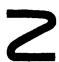
\includegraphics[keepaspectratio]{images/part001_a52dd4e1.jpg}}

\begin{enumerate}
\def\labelenumi{\arabic{enumi}.}
\setcounter{enumi}{5}
\item
  正文中的某些段落旨在预先提醒读者注意严重错误。这些段落在页边以（“危险弯道”）的标志标出。
\item
  习题既用于使读者检验自己是否已消化正文，也用于提醒读者注意那些不适合放入正文、但仍然有趣的结果。最困难的习题带有符号 Ⅱ。
\item
  一般而言，我们遵循公认的术语，除非有充分理由偏离它们。
\item
  我们特别努力始终使用严格正确的语言，同时不牺牲简明性。我们尽可能在正文中指出语言滥用；没有这些指出，任何数学文本都可能陷入迂腐，更不用说难以阅读。
\item
  由于原则上正文由某个理论的教条式阐述构成，通常不包含对文献的引用。书目引用汇集在历史注记中。每篇历史注记之后的书目通常只包括对所讨论理论的发展最为重要的著作和原始论文，并不声称以任何方式达到完整。
\end{enumerate}

至于习题，我们通常认为标明其来源没有价值，因为它们取自许多不同来源（原始论文、教科书、习题集）。

\begin{enumerate}
\def\labelenumi{\arabic{enumi}.}
\setcounter{enumi}{10}
\tightlist
\item
  本系列某一部分的引用方式如下：
\end{enumerate}

\begin{enumerate}
\def\labelenumi{\alph{enumi})}
\item
  如果引用的是同一节（§）中陈述的定理、公理或定义，则以其编号引用。
\item
  如果它们出现在同一章的另一节中，则引用中还要标明该节。
\item
  如果它们出现在同一部的另一章中，则标明该章和该节。
\item
  如果它们出现在另一部中，则首先用该部书名的缩写引用该部。
\end{enumerate}

结果汇总以字母 R 引用；因此，S, R 表示“集合论的结果汇总”。

\chapter{哈尔测度}

在本章和下一章中，当我们说到函数（分别地，测度）时，应理解为实函数或复函数（分别地，测度）；若 T 是局部紧空间，记号 \(\mathcal{K}(T)\) 将表示空间 \(\mathcal{K}_{\mathbf{R}}(T)\) 或空间 \(\mathcal{K}_{\mathbf{C}}(T)\)；对于记号 \(\overline{\mathcal{K}(T)}\)、\(\mathcal{C}(T)\)、\(L^{p}(T,\mu)\)、\(\mathcal{M}(T)\) 等也是如此。当然，在涉及多个函数、测度或向量空间的情形，所得结果在这些函数、测度或向量空间全为实的或全为复的时均成立。总是假定空间 \(\overline{\mathcal{K}(T)}\) 配备一致收敛拓扑，空间 \(\mathcal{C}(T)\) 配备紧收敛拓扑，空间 \(\mathcal{K}(T)\) 配备直接极限拓扑，其定义在第六章开头回顾。记号 \(\mathcal{K}_{+}(T)\) 表示满足 \(\geqslant0\) 的 \(\mathcal{K}(T)\) 函数集合。若 \(A\subset T\)，则 \(\varphi_{A}\) 总表示 A 的示性函数。若 \(t\in T\)，则 \(\varepsilon_{t}\) 表示在点 t 处质量为 +1 的正测度。

所有局部凸空间均假定为豪斯多夫空间。

除非明确另有说明，我们将 e 记为所考虑的所有群的单位元。

\section{哈尔测度的构造}

\subsection{定义与记号}

设 G 是在局部紧空间 X 上连续地左作用的拓扑群（GT, III, §2, No.~4）；对于 \(s \in G\) 和 \(x \in X\)，记 sx 为 s 对 x 的变换。我们用 \(\boldsymbol{\gamma}_{\mathbf{X}}(s)\) 或 \(\boldsymbol{\gamma}(s)\) 表示由下式定义的从 X 到 X 的同胚：

\[
\gamma (s) x = s x.\tag{1}
\]

有

\[
\boldsymbol {\gamma} (s t) = \boldsymbol {\gamma} (s) \boldsymbol {\gamma} (t).\tag{2}
\]

若 \(f\) 是定义在 \(X\) 上的函数，则 \(\boldsymbol{\gamma}(s)f\) 通过结构传递来定义，即令 \((\boldsymbol{\gamma}(s)f)(\boldsymbol{\gamma}(s)x) = f(x)\)；换言之，

\[
\big (\boldsymbol {\gamma} (s) f \big) (x) = f (s ^ {- 1} x).\tag{3}
\]

若 \(\mu\) 是定义在 X 上的测度，则 \(\gamma(s)\mu\) 也通过结构传递来定义，从而得到

\[
\langle f, \boldsymbol {\gamma} (s) \mu \rangle = \langle \boldsymbol {\gamma} (s ^ {- 1}) f, \mu \rangle \quad \text {   for   } f \in \mathscr {K} (\mathrm{X}).\tag{4}
\]

换言之，

\[
\int_ {\mathrm{X}} f (x) d (\boldsymbol {\gamma} (s) \mu) (x) = \int_ {\mathrm{X}} f (s x) d \mu (x).\tag{5}
\]

若 A 是 \((\gamma(s)\mu)\)-可积集，则 \(s^{-1}A\) 是 \(\mu\)-可积的，并且

\[
\left(\boldsymbol {\gamma} (s) \mu\right) (\mathrm{A}) = \mu \left(s ^ {- 1} \mathrm{A}\right).\tag{6}
\]

测度 \(\boldsymbol{\gamma}(s)\mu\) 也可以定义为 \(\mu\) 在 \(\boldsymbol{\gamma}(s)\) 下的像。有时，与其写作 \(d(\boldsymbol{\gamma}(s)\mu)(x)\)，不如写作 \(d\mu(s^{-1}x)\)；于是公式 (5) 变为：

\[
\int_ {\mathrm{X}} f (x) d \mu (s ^ {- 1} x) = \int_ {\mathrm{X}} f (s x) d \mu (x);
\]

右端的表达式于是可由左端通过“将 \(x\) 替换为 \(sx\)”得到。

定义 1. --- 设 \(\mu\) 是 X 上的一个测度。

\begin{enumerate}
\def\labelenumi{\alph{enumi})}
\item
  称 \(\mu\) 在 G 下不变，如果 \(\pmb{\gamma}(s)\mu = \mu\) 对每个 \(s\in \mathbf{G}\) 都成立。
\item
  称 \(\mu\) 在 \(\mathbf{G}\) 下相对不变，如果 \(\pmb{\gamma}(s)\pmb{\mu}\) 与 \(\pmb{\mu}\) 成比例对每个 \(s\in \mathbf{G}\) 都成立。
\item
  称 \(\mu\) 在 \(\mathbf{G}\) 下拟不变，如果 \(\pmb{\gamma}(s)\pmb{\mu}\) 与 \(\pmb{\mu}\) 等价对每个 \(s\in \mathbf{G}\) 都成立。
\end{enumerate}

评注。--- 1) 假设 \(\mu\) 不变。则 \(|\mu|\)、\(\mathcal{R}(\mu)\)、\(\mathcal{I}(\mu)\) 都是不变的。若 \(\mu\) 为实测度，则 \(\mu^{+}\) 和 \(\mu^{-}\) 也不变。

\begin{enumerate}
\def\labelenumi{\arabic{enumi})}
\setcounter{enumi}{1}
\tightlist
\item
  假设 \(\mu\) 相对不变且非零。对每个 \(s \in G\)，存在唯一的复数 \(\chi(s)\)，使得
\end{enumerate}

\[
\boldsymbol {\gamma} (s) \mu = \chi (s) ^ {- 1} \mu ,\tag{7}
\]

且函数 \(\chi\) 定义在 \(\mathbf{G}\) 上，是 \(\mathbf{G}\) 在 \(\mathbf{C}^*\) 中的表示，称为 \(\mu\) 的乘子。于是公式 (5) 给出

\[
\int_ {\mathrm{X}} f (s x) d \mu (x) = \chi (s) ^ {- 1} \int_ {\mathrm{X}} f (x) d \mu (x),\tag{8}
\]

而公式 (6) 给出

\[
\mu (s \mathrm{A}) = \chi (s) \mu (\mathrm{A}).\tag{9}
\]

按照上述约定，(7) 也可写成

\[
d \mu (s x) = \chi (s) d \mu (x).\tag{10}
\]

\begin{enumerate}
\def\labelenumi{\arabic{enumi})}
\setcounter{enumi}{2}
\tightlist
\item
  由于 \(|\pmb{\gamma}(s)\pmb{\mu}| = \pmb{\gamma}(s)(|\pmb{\mu}|)\)，说 \(\pmb{\mu}\) 拟不变，等价于说 \(|\pmb{\mu}|\) 拟不变。
\end{enumerate}

若 \(\mu\) 拟不变，且 \(\mu'\) 是 X 上与 \(\mu\) 等价的另一测度，则 \(\gamma(s)\mu'\) 与 \(\gamma(s)\mu\) 等价，因而与 \(\mu\) 等价，进而与 \(\mu'\) 等价，所以 \(\mu'\) 拟不变。因此，说 \(\mu\) 在 G 下拟不变，就是说 \(\mu\) 的等价类在 G 下不变。

\(\mu\) 拟不变的充要条件是：X 的局部 \(\mu\)-零测子集的集合在 G 下不变（Ch. V, §5, No.~5, Th. 2）；或者等价地，对 X 的每个 \(\mu\)-零测紧子集 K 及每个 \(s \in \mathbf{G}\)，sK 都是 \(\mu\)-零测的（同上，评注）。

若 \(\mu\) 拟不变，则 \(\mu\) 的支集在 G 下不变。特别地，若 G 在 X 上传递（A, I, §5, No.~5, Def. 6），则该支集或者为空（若 \(\mu = 0\)），或者等于 X（若 \(\mu \neq 0\)）。

引理 1. --- 设 X、Y、Z 是三个拓扑空间，其中 Y 局部紧。设 \((x,y)\mapsto xy\) 是从 \(X\times Y\) 到 Z 的连续映射，并定义映射 \(x\mapsto u_{x}\)，其值在 \(\mathcal{F}(Y;Z)\) 中，且满足关系 \(u_{x}(y)=xy\)。设 f 是 Z 上取值于 R 或某个巴拿赫空间的连续函数，S 是 f 的支集，\(\mu\) 是 Y 上的测度。假设对每个 \(x_{0}\in X\)，存在 X 中 \(x_{0}\) 的一个邻域 V，使得 \(\bigcup_{x\in V}u_{x}^{-1}(S)\) 在 Y 中相对紧。则：

\begin{enumerate}
\def\labelenumi{\alph{enumi})}
\tightlist
\item
  对每个 \(x \in X\)，\(f \circ u_{x}\) 都是 Y 上具有紧支集的连续函数；
\item
  由 a) 定义的映射 \(x \mapsto \int_{Y} f(xy) d\mu(y)\) 在 X 上连续。
\end{enumerate}

断言 a) 是显然的。证明 b)。由于连续性是局部性质，我们可以归结为 \(\bigcup_{x\in X}u_x^{-1}(S)\) 包含在 Y 的某个紧子集 \(Y'\) 中的情形。由于函数 \((x,y)\mapsto f(xy)\) 在 \(X\times Y\) 上连续，\(f\circ u_x\) 一致趋于 \(f\circ u_{x_0}\)（在 \(Y'\) 上，当 \(x\) 趋于 \(x_0\) 时），（GT, X, §3, No.~4, Th. 3），因此 \(\mu(f \circ u_x)\) 趋于 \(\mu(f \circ u_{x_0})\)。引理得证。

现在回到前面的记号。

命题 1. --- 假设 G 局部紧。设 \(\mu\) 是 X 上非零的相对不变测度。则其乘子 \(\chi\) 是 G 上的连续函数。

事实上，取 \(f \in \mathcal{K}(\mathbf{X})\)，令 \(S\) 为 \(f\) 的支集，令 \(s_0\) 为 \(G\) 中一点，并令 \(V\) 为 \(s_0\) 在 \(G\) 中的紧邻域；则集合

\[
\bigcup_ {s \in V} \gamma (s) ^ {- 1} (S) = V ^ {- 1} S
\]

在 X 中是紧的；由引理 1 和公式 (8)，\(\chi(s^{-1})\langle\mu, f\rangle\) 连续依赖于 \(s\)；若选取 \(f\) 使得 \(\langle\mu, f\rangle \neq 0\)，便知 \(\chi\) 连续。

现在设 G 是在局部紧空间 X 上连续地右作用的拓扑群；对于 \(s \in G\) 和 \(x \in X\)，记 xs 为 s 对 x 的变换。我们用 \(\delta_{\mathbf{X}}(s)\) 或 \(\delta(s)\) 表示由下式定义的 X 上的同胚：

\[
\delta (s) x = x s ^ {- 1}.\tag{1'}
\]

有

\[
\boldsymbol {\delta} (s t) = \boldsymbol {\delta} (s) \boldsymbol {\delta} (t).\tag{2'}
\]

通过结构传递，定义 \(\boldsymbol{\delta}(s)\) 在 X 上的函数和测度上的作用：



\[
\big (\boldsymbol {\delta} (s) f \big) (x) = f (x s)\tag{3'}
\]

\[
\langle f, \delta (s) \mu \rangle = \langle \delta (s ^ {- 1}) f, \mu \rangle\tag{4'}
\]

\[
\int_ {\mathrm{X}} f (x) d \bigl (\pmb {\delta} (s) \mu \bigr) (x) = \int_ {\mathrm{X}} f (x s ^ {- 1}) d \mu (x)\tag{5'}
\]

\[
\big (\delta (s) \mu \big) (\mathrm{A}) = \mu (\mathrm{A} s).\tag{6'}
\]

我们约定用 \(d\mu(xs)\) 代替 \(d(\pmb{\delta}(s)\mu)(x)\)，于是 \((5')\) 变为

\[
\int_ {\mathrm{X}} f (x) d \mu (x s) = \int_ {\mathrm{X}} f (x s ^ {- 1}) d \mu (x).
\]

以类似方式定义 X 上在 G 下不变、相对不变和拟不变的测度。若 \(\mu\) 相对不变，则其乘子 \(\chi\) 由下列公式定义：



\[
\boldsymbol {\delta} (s) \mu = \chi (s) \mu\tag{7'}
\]

\[
\int_ {\mathrm{X}} f (x s) d \mu (x) = \chi (s) ^ {- 1} \int_ {\mathrm{X}} f (x) d \mu (x)\tag{8'}
\]

\[
\mu (\mathrm{A} s) = \chi (s) \mu (\mathrm{A})\tag{9'}
\]

\[
d \mu (x s) = \chi (s) d \mu (x).\tag{10'}
\]

若把与 G 对立的群 \(G^{0}\) 看作通过 \((x, s) \mapsto xs\) 作用于 X，则 \(\mu\) 在 \(G^{0}\) 下相对不变，且乘子仍为 \(\chi\)。

最后，设 \(\mathbf{G}\) 是局部紧群。按照公式 \(\pmb{\gamma}(s)x = sx\)、\(\pmb{\delta}(s)x = xs^{-1}\)，它通过左平移和右平移作用于自身。于是

\[
\boldsymbol {\gamma} (s) \boldsymbol {\delta} (t) = \boldsymbol {\delta} (t) \boldsymbol {\gamma} (s).\tag{11}
\]

以上一切在此均适用，因此在 G 上我们有左不变、右不变、相对左不变、相对右不变、左拟不变和右拟不变测度的概念（不过见第 8、9 号）。

映射 \(x \mapsto x^{-1}\) 是从 \(G\) 到 \(G\) 的同胚。对于函数 \(f\)（定义在 \(G\) 上），定义函数 \(\overset{\vee}{f}\)（在 \(G\) 上）：

\[
\stackrel {\vee} {f} (x) = f (x ^ {- 1}).\tag{12}
\]

对于测度 \(\mu\)（定义在 \(\mathbf{G}\) 上），定义测度 \(\breve{\mu}\)：

\[
\stackrel {\vee} {\mu} (f) = \mu (\stackrel {\vee} {f}) \quad \text { for } f \in \mathcal {K} (\mathrm{G}).\tag{13}
\]

换言之，

\[
\int_ {\mathrm{G}} f (x) d \mu^ {\vee} (x) = \int_ {\mathrm{G}} f (x ^ {- 1}) d \mu (x).\tag{14}
\]

若 \(\mathbf{A}\) 是 \(\check{\mu}\)-可积集，则 \(\mathbf{A}^{-1}\) 是 \(\mu\)-可积的，并且

\[
\check {\mu} (\mathrm{A}) = \mu (\mathrm{A} ^ {- 1}).\tag{15}
\]

我们约定用 \(d\mu(x^{-1})\) 代替 \(d\check{\mu}(x)\)，于是 (14) 变为

\[
\int_ {\mathrm{G}} f (x) d \mu (x ^ {- 1}) = \int_ {\mathrm{G}} f (x ^ {- 1}) d \mu (x).
\]

\subsection{存在性与唯一性定理}

定义 2. --- 设 G 是局部紧群。G 上非零且左（分别地，右）不变的正测度称为 G 上的左（分别地，右）哈尔测度。

定理 1. --- 每个局部紧群上都存在左（分别地，右）哈尔测度，并且除相差一个常数因子外只有一个。

\begin{enumerate}
\def\labelenumi{\Alph{enumi})}
\tightlist
\item
  存在性。--- 置 \(\mathcal{K}(\mathrm{G}) = \mathcal{K}\)、\(\mathcal{K}_{+}(\mathrm{G}) = \mathcal{K}_{+}\)、\(\mathcal{K}_{+}^{*} = \mathcal{K}_{+} - \{0\}\)。若 C 是 G 的紧子集，则以 \(\mathcal{K}_{+}^{*}(\mathrm{C})\) 表示支集包含在 C 中的 \(f \in \mathcal{K}_{+}^{*}\) 的集合。对于 \(f \in \mathcal{K}\) 和 \(g \in \mathcal{K}_{+}^{*}\)，存在数 \(c_{1}, \ldots, c_{n} \geqslant 0\) 以及 G 中的元素 \(s_{1}, \ldots, s_{n}\)，使得 \(f \leqslant \sum_{i=1}^{n} c_{i} \gamma(s_{i}) g\)：这是因为，G 中存在非空开集 U，使得 \(\inf_{s \in \mathrm{U}} g(s) > 0\)，并且 \(f\) 的支集可以被 U 的有限个左平移覆盖。令 \((f : g)\) 为数 \(\sum_{i=1}^{n} c_{i}\) 的下确界，其中所有系统 \((c_{1}, \ldots, c_{n}, s_{1}, \ldots, s_{n})\) 由数 \(\geqslant 0\) 和 G 中的元素组成，并满足 \(f \leqslant \sum_{i=1}^{n} c_{i} \gamma(s_{i}) g\)。则：
\end{enumerate}

\begin{enumerate}
\def\labelenumi{(\roman{enumi})}
\item
  \(\left(\pmb{\gamma}(s)f:g\right) = (f:g)\) 对于 \(f\in \mathcal{K}\)、\(g\in \mathcal{K}_{+}^{*}\)、\(s\in G\) 成立；
\item
  \((\lambda f:g) = \lambda (f:g)\) 对于 \(f\in \mathcal{K}\) \(,g\in \mathcal{K}_{+}^{*},\lambda \geqslant 0\) 成立。
\item
  \(\left((f + f^{\prime}):g\right)\leqslant (f:g) + (f^{\prime}:g)\) 对于 \(f\in \mathcal{K},f^{\prime}\in \dot{\mathcal{K}},g\in \mathcal{K}_{+}^{*};\) 成立；
\item
  有 \((f:g)\geqslant (\sup f) / (\sup g)\)。
\end{enumerate}

\[
f \in \mathscr {K}, g \in \mathscr {K} _ {+} ^ {*}
\]

\begin{enumerate}
\def\labelenumi{(\alph{enumi})}
\setcounter{enumi}{21}
\tightlist
\item
  \((f:h)\leqslant (f:g)(g:h)\) 对于 \(f\in \mathcal{K}\) \(,g\in \mathcal{K}_{+}^{*}\) \(h\in \mathcal{K}_{+}^{*};\) 成立；
\end{enumerate}

\begin{enumerate}
\def\labelenumi{(\roman{enumi})}
\setcounter{enumi}{5}
\item
  \(0 < \frac{1}{(f_0:f)}\leqslant \frac{(f:g)}{(f_0:g)}\leqslant (f:f_0)\) 对于 \(f,f_0,g\) 属于 \(\mathcal{K}_+^*\) 成立；
\item
  设 \(f, f', h\) 属于 \(\mathcal{K}_+\)，且 \(h(s) \geqslant 1\) 在 \(f + f'\) 的支集上成立，再设 \(\varepsilon > 0\)；存在一个紧邻域 \(V\)，以 \(e\) 为中心，使得对每个 \(g \in \mathcal{K}_+^*(V)\)，
\end{enumerate}

\[
(f: g) + (f ^ {\prime}: g) \leqslant ((f + f ^ {\prime}): g) + \varepsilon (h: g).
\]

性质 (i)、(ii)、(iii) 显然。取 \(f \in \mathcal{K}\)、\(g \in \mathcal{K}_+^*\)；若 \(f \leqslant \sum_{i=1}^{n} c_i \gamma(s_i)g\)，且 \(c_i \geqslant 0\)，则 \(\sup f \leqslant \sum_{i=1}^{n} c_i g(s_i^{-1}s)\) 对某个 \(s \in \mathbf{G}\) 成立，因而 \(\sup f \leqslant \left( \sum_{i=1}^{n} c_i \right) \sup g\)，从而得到 (iv)。现在证明 (v)；取 \(f \in \mathcal{K}\)、\(g, h\) 属于 \(\mathcal{K}_+^*\)；若 \(f \leqslant \sum_{i=1}^{n} c_i \boldsymbol{\gamma}(s_i) g\) 且 \(g \leqslant \sum_{j=1}^{p} d_j \boldsymbol{\gamma}(t_j) h\)（\(c_i \geqslant 0\)、\(d_j \geqslant 0\)、\(s_i, t_j\) 属于 G），则 \(f \leqslant \sum_{i,j} c_i d_j \boldsymbol{\gamma}(s_i t_j) h\)，故 \((f: h) \leqslant \sum_{i,j} c_i d_j = \left( \sum_{i} c_i \right) \left( \sum_{j} d_j \right)\)；于是 \((f: h) \leqslant (f: g)(g: h)\)。把 (v) 一方面应用于 \(f_0, f, g\)，另一方面应用于 \(f, f_0, g\)，得到 (vi)。最后，设 \(f, f', h\) 属于 \(\mathcal{K}_+\)，且 \(h(s) \geqslant 1\) 在 \(f + f'\) 的支集上成立，再设 \(\varepsilon > 0\)。令 \(\mathbf{F} = f + f' + \frac{1}{2} \varepsilon h\)；函数 \(\varphi, \varphi'\) 分别与 \(f / F\) 和 \(f'/F\) 一致于 \(f + f'\) 的支集上，并在其外为零，属于 \(\mathcal{K}_+\)；对每个 \(\eta > 0\)，存在一个紧邻域 V，以 \(e\) 为中心，使得 \(|\varphi(s) - \varphi(t)| \leqslant \eta\) 且 \(|\varphi'(s) - \varphi'(t)| \leqslant \eta\) 在 \(s^{-1} t \in V\) 时成立。于是取 \(g \in \mathcal{K}_+^*(V)\)；对每个 \(s \in G\)，

\[
\varphi \cdot \boldsymbol {\gamma} (s) g \leqslant (\varphi (s) + \eta) \cdot \boldsymbol {\gamma} (s) g;
\]

这是因为，在 \(\pmb{\gamma}(s)g\) 为零的点，即在 \(s\mathbf{V}\) 之外，该不等式显然成立；而在 \(s\mathbf{V}\) 内，\(\varphi \leqslant \varphi(s) + \eta\)；同样，\(\varphi' \cdot \pmb{\gamma}(s)g \leqslant (\varphi'(s) + \eta) \cdot \pmb{\gamma}(s)g\)。现设数 \(c_1, \ldots, c_n\) 满足 \(\geqslant 0\)，并设 \(s_1, \ldots, s_n\) 为 \(\mathbf{G}\) 中的元素，使得 \(\mathbf{F} \leqslant \sum_{i=1}^{n} c_i \pmb{\gamma}(s_i)g\)；则

\[
f = \varphi \mathrm{F} \leqslant \sum_ {i = 1} ^ {n} c _ {i} \varphi \cdot \boldsymbol {\gamma} (s _ {i}) g \leqslant \sum_ {i = 1} ^ {n} c _ {i} (\varphi (s _ {i}) + \eta) \cdot \boldsymbol {\gamma} (s _ {i}) g
\]

对 \(f'\) 同理；因此

\[
(f: g) + (f ^ {\prime}: g) \leqslant \sum_ {i = 1} ^ {n} c _ {i} (\varphi (s _ {i}) + \varphi^ {\prime} (s _ {i}) + 2 \eta) \leqslant (1 + 2 \eta) \sum_ {i = 1} ^ {n} c _ {i}
\]

因为 \(\varphi +\varphi^{\prime}\leqslant 1\)。应用 F 的定义，再应用 (ii)、(iii) 和 (v)，可得

\[
\begin{array}{r l} & {(f: g) + (f ^ {\prime}: g) \leqslant (1 + 2 \eta) (\mathrm{F}: g) \leqslant} \\ & {\quad (1 + 2 \eta) \big [ \big ((f + f ^ {\prime}): g \big) + \frac {1}{2} \varepsilon (h: g) \big ] \leqslant} \\ & {\quad \big ((f + f ^ {\prime}): g \big) + \frac {1}{2} \varepsilon (h: g) + 2 \eta \big ((f + f ^ {\prime}): h \big) (h: g) + \varepsilon \eta (h: g)} \end{array}
\]

并且，若选择 \(\eta\) 使得 \(\eta\big[2\big((f + f'):h\big) + \varepsilon\big] \leqslant \frac{1}{2}\varepsilon\)，则得到 (vii)。

当 V 遍历 \(e\) 的紧邻域集合时，\(\mathcal{K}_{+}^{*}(V)\) 构成滤子 \(\mathfrak{B}\) 在 \(\mathcal{K}_{+}^{*}\) 上的一个基。令 \(\mathfrak{F}\) 为 \(\mathcal{K}_{+}^{*}\) 上比 \(\mathfrak{B}\) 更细的超滤子。另一方面，固定 \(f_{0} \in \mathcal{K}_{+}^{*}\)，并对 \(f \in \mathcal{K}_{+}^{*}\) 和 \(g \in \mathcal{K}_{+}^{*}\) 置

\[
\mathrm{I} _ {g} (f) = \frac {(f : g)}{(f _ {0} : g)}.
\]

由 (vi)，\(\lim_{g,\mathfrak{F}}\mathrm{I}_g(f) = \mathrm{I}(f)\) 存在于紧空间 \([1 / (f_0:f),(f:f_0)]\) 中。由 (iii)，\(\mathrm{I}(f + f')\leqslant \mathrm{I}(f) + \mathrm{I}(f')\)。由 (vii)，\(\mathrm{I}(f) + \mathrm{I}(f')\leqslant \mathrm{I}(f + f') + \varepsilon \mathrm{I}(h)\) 对所有 \(\varepsilon >0\) 成立，只要 \(h\) 满足 \(\geqslant 1\) 于 \(f + f'\) 的支集上；由此 \(\mathrm{I}(f + f') = \mathrm{I}(f) + \mathrm{I}(f')\)。根据 Ch. II, §2, No.~1, Prop. 2，I 可延拓为 \(\mathcal{K}\) 上的线性形式；该线性形式是 G 上的非零正测度，并由 (i) 左不变；这就是所求的左哈尔测度。转到对立群即可推出右哈尔测度的存在。

\begin{enumerate}
\def\labelenumi{\Alph{enumi})}
\setcounter{enumi}{1}
\tightlist
\item
  唯一性。--- 设 \(\mu\) 为左哈尔测度，\(\nu\) 为右哈尔测度。则 \(\check{\nu}\) 是左哈尔测度。我们将证明 \(\mu\) 与 \(\check{\nu}\) 成比例。这将证明任意两个左哈尔测度确实成比例。
\end{enumerate}

取 \(f \in \mathcal{K}\) 使得 \(\mu(f) \neq 0\)。由引理 1，按下式定义的函数 \(D_f\) 在 \(G\) 上

\[
\mathrm{D} _ {f} (s) = \mu (f) ^ {- 1} \int f (t ^ {- 1} s) d \nu (t)\tag{16}
\]

在 G 上连续。取 \(g \in \mathcal{K}\)。函数 \((s, t) \mapsto f(s)g(ts)\) 在 G × G 中连续且具有紧支集。由 Ch. III, §4, No.~1, Th. 2，

\[
\begin{array}{r l} & {\mu (f) \nu (g) = \Big (\int f (s) d \mu (s) \Big) \Big (\int g (t) d \nu (t) \Big)} \\ & {\qquad = \int d \mu (s) \int f (s) g (t s) d \nu (t) = \int d \nu (t) \int f (s) g (t s) d \mu (s)} \\ & {\qquad = \int d \nu (t) \int f (t ^ {- 1} s) g (s) d \mu (s)} \\ & {\qquad = \int g (s) \Big [ \int f (t ^ {- 1} s) d \nu (t) \Big ] d \mu (s) = \mu \big (g \cdot \mu (f) D _ {f} \big),} \end{array}\tag{17}
\]

从而

\[
\nu (g) = \mu (\mathrm{D} _ {f} \cdot g).\tag{18}
\]

首先，这证明 \(D_{f}\) 与 f 无关。对于 \(f' \in H\)，若满足 \(\mu(f') \neq 0\)，则有 \(D_{f} \cdot \mu = D_{f'} \cdot \mu\)，因此 \(D_{f} = D_{f'}\) 在 \(\mu\) 下局部几乎处处成立，进而处处成立，因为 \(\mathbf{D}_f\) 和 \(\mathbf{D}_{f'}\) 连续且 \(\mu\) 的支集为 \(\mathbf{G}\)。因此可记 \(\mathrm{D}_f = \mathrm{D}\)。公式 (16) 给出

\[
\mu (f) \mathrm{D} (e) = \stackrel {\vee} {\nu} (f).\tag{19}
\]

公式 (19) 可通过线性延拓到函数 \(f \in \mathcal{K}\)，其中满足 \(\mu(f) = 0\)。有 \(D(e) \neq 0\)，因为 \(\check{\nu} \neq 0\)。这就确立了 \(\mu\) 与 \(\check{\nu}\) 的比例关系。

推论。--- G 上每个左不变（分别地，右不变）测度都与某个左（分别地，右）哈尔测度成比例。

例。--- 1) 在加法群 R 上，勒贝格测度 dx 是哈尔测度（Ch. III, §1, No.~3, 例）。

\begin{enumerate}
\def\labelenumi{\arabic{enumi})}
\setcounter{enumi}{1}
\tightlist
\item
   对于每个函数 \(f \in \mathcal{K}(\mathbf{R}_+^*)\)，有（FRV, II, §1, 公式 (12)）
\end{enumerate}

\[
\int_ {0} ^ {+ \infty} \frac {f (x)}{x} d x = \int_ {0} ^ {+ \infty} \frac {f (t x)}{t x} t d x = \int_ {0} ^ {+ \infty} \frac {f (t x)}{x} d x
\]

对所有 t \textgreater{} 0，测度 \(x^{-1} dx\) 因而是乘法群 \(R_{+}^{*}\) 上的哈尔测度。

\begin{enumerate}
\def\labelenumi{\arabic{enumi})}
\setcounter{enumi}{2}
\tightlist
\item
  取 G 为圆环 \(\mathbf{T} = \mathbf{R} / \mathbf{Z}\)。令 \(\varphi\) 为从 \(\mathbf{R}\) 到 \(\mathbf{T}\) 的典范映射。对于 \(f \in \mathcal{K}(\mathbf{T})\)，函数 \(f \circ \varphi\) 在 \(\mathbf{R}\) 上连续且以 1 为周期，积分
\end{enumerate}

\[
\mathrm{I} (f) = \int_ {a} ^ {a + 1} f (\varphi (x)) d x
\]

与 \(a \in \mathbf{R}\) 的选择无关；它显然关于平移不变；因此它定义了 \(\mathbf{T}\) 上的哈尔测度。通过结构传递，由此得到 \(I(f) = \int_{a}^{a + 1} f(e^{2\pi it}) dt\) 是复数绝对值为 1 的乘法群 \(\mathbf{U}\) 上的哈尔测度（GT, VIII, §2, No.~1）。

命题 2. --- 设 G 是局部紧群，\(\mu\) 是 G 上的左或右哈尔测度。G 为离散的充要条件是 \(\mu(\{e\}) > 0\)。G 为紧的充要条件是 \(\mu^{*}(G) < +\infty\)。

这些条件显然是必要的。证明它们的充分性。令 V 为 e 的紧邻域。若 \(\mu(\{e\}) > 0\)，则由于 \(\mu(V) < +\infty\)，V 是有限集；由于 G 是豪斯多夫空间，因而 G 是离散的。假设 \(\mu^{*}(G)<+\infty\)，并且例如 \(\mu\) 左不变。考虑集合 \(\mathscr{E}\)，它由 G 的有限子集 \(\{s_{1},\ldots,s_{n}\}\) 组成，且满足 \(s_{i}V\cap s_{j}V=\varnothing\) 当 \(i\neq j\) 时；则

\[
n \mu (\mathrm{V}) = \mu (s _ {1} \mathrm{V} \cup \dots \cup s _ {n} \mathrm{V}) \leqslant \mu^ {*} (\mathrm{G}),
\]

因此 \(n \leqslant \mu^{*}(\mathrm{G})/\mu(\mathrm{V})\)。于是可以在 E 中选取一个极大元 \(\{s_{1},\ldots,s_{n}\}\)。然后，对于每个 \(s \in G\)，存在某个 i 使得 \(sV \cap s_{i}V \neq \varnothing\)，从而有 \(s \in s_{i}VV^{-1}\)。因此 G 是紧集 \(s_{i}VV^{-1}\) 的并，故为紧的。

\subsection{模}

设 \(\mu\) 是 G 上的左哈尔测度。对于每个 \(s \in \mathbf{G}\)，\(\pmb{\delta}(s)\mu\) 也是左不变的（No.~1, 公式 (11)），因此由定理 1，存在唯一的数 \(\Delta_{\mathbf{G}}(s) > 0\)，使得 \(\pmb{\delta}(s)\mu = \Delta_{\mathbf{G}}(s)\mu\)。根据定理 1，数 \(\Delta_{\mathbf{G}}(s)\) 与 \(\mu\) 的选择无关。

定义 3. --- 函数 \(\Delta_{\mathbf{G}}\) 定义在 \(\mathbf{G}\) 上，称为 \(\mathbf{G}\) 的模（或模函数）。若 \(\Delta_{\mathbf{G}} = 1\)，则称群 \(\mathbf{G}\) 为幺模群。

也可以说 \(\mu\) 是右相对不变的，乘子为 \(\Delta_{\mathbf{G}}\)。因此 \(\Delta_{\mathbf{G}}\) 是 \(\mathbf{G}\) 在 \(\mathbf{R}_{+}^{*}\) 中的连续表示（No.~1, Prop. 1）。

评注。--- 若 \(\varphi\) 是从 \(G\) 到局部紧群 \(G'\) 的同构，则 \(\Delta_{G'} \circ \varphi = \Delta_G\)。特别地：

\begin{enumerate}
\def\labelenumi{\arabic{enumi})}
\item
  由于 \(x \mapsto x^{-1}\) 是从 \(G\) 到对立群 \(G^0\) 的同构，有 \(\Delta_{G^0} = \Delta_{G}^{-1}\)。
\item
  若 \(\varphi\) 是 \(G\) 的自同构，则 \(\Delta_G \circ \varphi = \Delta_G\)。
\end{enumerate}

取 \(s \in G\)。则：

\[
\boldsymbol {\delta} (s) \left(\Delta_ {\mathrm{G}} ^ {- 1} \cdot \mu\right) = \left(\boldsymbol {\delta} (s) \Delta_ {\mathrm{G}} ^ {- 1}\right) \cdot \left(\boldsymbol {\delta} (s) \mu\right) = \left(\Delta_ {\mathrm{G}} (s) ^ {- 1} \Delta_ {\mathrm{G}} ^ {- 1}\right) \cdot \left(\Delta_ {\mathrm{G}} (s) \mu\right) = \Delta_ {\mathrm{G}} ^ {- 1} \cdot \mu ,
\]

因此 \(\Delta_{\mathrm{G}}^{-1} \cdot \mu = \mu'\) 是右哈尔测度。由此可得 \(\boldsymbol{\gamma}(s)\mu' = (\boldsymbol{\gamma}(s)\Delta_{\mathrm{G}}^{-1}) \cdot \mu = \Delta_{\mathrm{G}}(s)(\Delta_{\mathrm{G}}^{-1} \cdot \mu) = \Delta_{\mathrm{G}}(s)\mu'\)，所以对于每个右哈尔测度 \(\nu\)，都有 \(\boldsymbol{\gamma}(s)\nu = \Delta_{\mathrm{G}}(s)\nu\)。由于 \(\breve{\mu}\) 是右哈尔测度，有 \(\breve{\mu} = a\Delta_{\mathrm{G}}^{-1} \cdot \mu\)，其中常数 \(a > 0\)；于是

\[
\mu = a \big (\Delta_ {\mathrm{G}} ^ {- 1} \cdot \mu \big) ^ {\vee} = a \Delta_ {\mathrm{G}} \cdot \stackrel {\vee} {\mu} = a ^ {2} \mu ,
\]

因此 \(a = 1\)，最后 \(\check{\mu} = \Delta_{\mathrm{G}}^{-1}\cdot \mu\)。同理可得 \(\check{\nu} = \Delta_{\mathrm{G}}\cdot \nu\)。因此有以下结果：

公式表。--- 设 G 是局部紧群，\(\Delta\) 是其模，\(\mu\) 是左哈尔测度，\(\nu\) 是右哈尔测度。

\begin{enumerate}
\def\labelenumi{\arabic{enumi})}
\tightlist
\item
  有
\end{enumerate}

\[
\boldsymbol {\gamma} (s) \mu = \mu \quad \boldsymbol {\delta} (s) \mu = \Delta (s) \mu \quad \check {\mu} = \Delta^ {- 1} \cdot \mu .\tag{20}
\]

若 \(f\) 在 \(\mu\) 下于 \(G\) 可积，则 \(f\) 的左、右平移也在 \(\mu\) 下可积，并且

\[
\begin{array}{l} \int f (s x) d \mu (x) = \int f (x) d \mu (x) \\ \int f (x s) d \mu (x) = \Delta (s) ^ {- 1} \int f (x) d \mu (x). \end{array}\tag{21}
\]

此外，\(\stackrel{\vee}{f}\) 对 \(\Delta^{-1} \cdot \mu\) 可积，并且

\[
\int f (x ^ {- 1}) \Delta (x) ^ {- 1} d \mu (x) = \int f (x) d \mu (x).\tag{22}
\]

若 A 是 G 的 \(\mu\)-可积子集，则 sA 和 As 也在 \(\mu\) 下可积，并且

\[
\mu (s \mathrm{A}) = \mu (\mathrm{A}) \quad \mu (\mathrm{A} s) = \Delta (s) \mu (\mathrm{A}).\tag{23}
\]

\begin{enumerate}
\def\labelenumi{\arabic{enumi})}
\setcounter{enumi}{1}
\tightlist
\item
  有
\end{enumerate}

\[
\boldsymbol {\delta} (s) \nu = \nu \quad \boldsymbol {\gamma} (s) \nu = \Delta (s) \nu \quad \check {\nu} = \Delta \cdot \nu .\tag{24}
\]

若 \(f\) 在 \(\nu\) 下于 \(G\) 可积，则 \(f\) 的左、右平移也在 \(\nu\) 下可积，并且

\[
\begin{array}{l} \int f (x s) d \nu (x) = \int f (x) d \nu (x) \\ \int f (s x) d \nu (x) = \Delta (s) \int f (x) d \nu (x). \end{array}\tag{25}
\]

此外，\(\stackrel{\vee}{f}\) 对 \(\Delta \cdot \nu\) 可积，并且

\[
\int f (x ^ {- 1}) \Delta (x) d \nu (x) = \int f (x) d \nu (x).\tag{26}
\]

若 A 是 G 的 \(\nu\)-可积子集，则 sA 和 As 也在 \(\nu\) 下可积，并且

\[
\nu (\mathrm{A} s) = \nu (\mathrm{A}) \quad \nu (s \mathrm{A}) = \Delta (s) ^ {- 1} \nu (\mathrm{A}).\tag{27}
\]

\begin{enumerate}
\def\labelenumi{\arabic{enumi})}
\setcounter{enumi}{2}
\item
  \(\nu\) 与 \(\Delta^{-1} \cdot \mu\) 成比例，且 \(\mu\) 与 \(\Delta \cdot \nu\) 成比例。
\item
  假设 G 是幺模的。令 \(\mu\) 为 G 上的哈尔测度。则：
\end{enumerate}

\[
\boldsymbol {\gamma} (s) \mu = \boldsymbol {\delta} (s) \mu = \stackrel {\vee} {\mu} = \mu .\tag{28}
\]

若 \(f\) 在 \(\mu\) 下于 \(G\) 可积，则 \(f\) 的左、右平移也在 \(\mu\) 下可积，\(\overset{\vee}{f}\) 亦然，并且

\[
\int f (s x) d \mu (x) = \int f (x s) d \mu (x) = \int f (x ^ {- 1}) d \mu (x) = \int f (x) d \mu (x).\tag{29}
\]

若 \(\mathbf{A}\) 是 \(\mu\) 下在 \(\mathbf{G}\) 中可积的子集，则 \(s\mathbf{A}\)、\(\mathbf{A}s\) 和 \(\mathbf{A}^{-1}\) 都在 \(\mu\) 下可积，并且

\[
\mu (s \mathrm{A}) = \mu (\mathrm{A} s) = \mu (\mathrm{A} ^ {- 1}) = \mu (\mathrm{A}).\tag{30}
\]

本质积分也具有相应的性质。

命题 3. --- 若 G 中存在一个在内自同构下不变的 e 的紧邻域 V，则 G 是幺模的。

事实上，设 \(\mu\) 是 \(\mathbf{G}\) 上的左哈尔测度。对于每个 \(s \in \mathbf{G}\)，

\[
\mu (\mathrm{V}) = \mu (s ^ {- 1} \mathrm{Vs}) = \Delta_ {\mathrm{G}} (s) \mu (\mathrm{V}),
\]

从而 \(\Delta_{\mathbf{G}}(s) = 1\)，因为 \(0 < \mu (\mathrm{V}) < +\infty\)。

由此立即得到：

推论。--- 若 G 是离散的、紧的或交换的，则 G 是幺模的。

当 G 交换时，这一点更是显然的。还要注意，若 G 是离散的，则 G 上每个点质量为 1 的测度显然是 G 上的左、右哈尔测度，称为 G 上的归一化哈尔测度。若 G 是紧的，则 G 上存在唯一满足 \(\mu(G)=1\) 的哈尔测度，称为 G 的归一化哈尔测度。当前两种约定同时适用于 G 既离散又紧、即有限的情形时，它们并不一致；在这种情况下，我们总会明确说明“归一化哈尔测度”的含义。

\pandocbounded{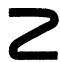
\includegraphics[keepaspectratio]{images/part001_35d0c9a3.jpg}}

幺模群的子群和商群不一定幺模（\(\S2\)，习题 5）。不过参见 \(\S2\) 的命题 10, No.~7。

*稍后我们将看到，半单或幂零连通李群是幺模的。*

\subsection{自同构的模}

设 G 是局部紧群，\(\varphi\) 是 G 的自同构，\(\mu\) 是 G 上的左哈尔测度。显然，\(\varphi^{-1}(\mu)\) 也是 G 上的左哈尔测度。因此存在（No.~2, Th. 1）唯一的数 a \textgreater{} 0，使得 \(\varphi^{-1}(\mu) = a\mu\)。根据 No.~2, Th. 1，该数与 \(\mu\) 的选择无关。注意，若一开始取右哈尔测度，例如 \(\Delta_{G}^{-1} \cdot \mu\)（No.~3），也会得到同一个标量 a：因为 \(\varphi^{-1}\) 保持 \(\Delta_{G}\) 不变（No.~3, 评注），有 \(\varphi^{-1}(\Delta_{G}^{-1} \cdot \mu) = \Delta_{G}^{-1} \cdot \varphi^{-1}(\mu) = a\Delta_{G}^{-1} \cdot \mu\)。

定义 4. --- 数 a \textgreater{} 0 满足 \(\varphi^{-1}(\mu) = a\mu\)，称为自同构 \(\varphi\) 的模，记为 mod G \(\varphi\)，或简称为 mod \(\varphi\)。

若 \(f\) 是在 \(\mu\) 下于 \(G\) 可积的函数，则

\[
\int f \big (\varphi^ {- 1} (x) \big) d \mu (x) = (\mathrm{mod} \varphi) \int f (x) d \mu (x).\tag{31}
\]

若 A 是 G 的 \(\mu\)-可积子集，则

\[
\mu (\varphi (\mathrm{A})) = (\mathrm{mod} \varphi) \mu (\mathrm{A}).\tag{32}
\]

特别地，对于 \(s \in \mathbf{G}\)，令 \(i_s\) 为内自同构 \(x \mapsto s^{-1}xs\)。则 \(i_s^{-1} = \delta(s)\gamma(s)\)，因而

\[
i _ {s} ^ {- 1} (\mu) = \delta (s) \mu = \Delta_ {\mathrm{G}} (s) \mu ,
\]

所以

\[
\operatorname{mod} i _ {s} = \Delta_ {\mathrm{G}} (s).\tag{33}
\]

若 G 是离散群或紧群，则其归一化哈尔测度在 G 的每个自同构 \(\varphi\) 下都变为自身，这由结构传递立即可见。因此，离散群或紧群的自同构的模为 1。

命题 4. --- 设 G 是局部紧群，\(\Gamma\) 是拓扑群，且 \(\gamma \mapsto u_{\gamma}\) 是从 \(\Gamma\) 到 G 的自同构群 \(\mathcal{G}\) 的同态，并满足 \((\gamma, x) \mapsto u_{\gamma}(x)\) 是从 \(\Gamma \times G\) 到 G 的连续映射。则映射 \(\gamma \mapsto \operatorname{mod}(u_{\gamma})\) 是 \(\Gamma\) 在 \(\mathbf{R}_{+}^{*}\) 中的连续表示。

这个映射显然是 \(\Gamma\) 在 \(\mathbf{R}_+^*\) 中的（代数）表示；只需证明其连续性。取 \(f \in \mathcal{K}(\mathbf{G})\)，令 \(\mathbf{S}\) 为其支集。

取 \(\gamma_0 \in \Gamma\)，令 \(U\) 为 \(u_{\gamma_0}^{-1}(S)\) 的相对紧邻域。映射 \(\gamma \mapsto u_\gamma\) 是从 \(\Gamma\) 到赋予紧收敛拓扑的 \(\mathcal{G}\) 的连续映射（GT, X, §3, No.~4, Th. 3）；因此，\(u_{\gamma}^{-1}(S) \subset U\) 在 \(\gamma\) 充分接近 \(\gamma_0\) 时成立。No.~1 的引理 1 于是证明 \(\int f(u_\gamma(x)) d\mu(x)\)（其中 \(\mu\) 表示 \(G\) 上的左哈尔测度）连续依赖于 \(\gamma\)；命题得证。

\subsection{乘积的哈尔测度}

命题 5. --- 设 \((\mathbf{G}_{\iota})_{\iota \in \mathbf{I}}\) 是局部紧群的一个族。对每个 \(\iota \in \mathbf{I}\)，令 \(\mu_{\iota}\) 为 \(\mathbf{G}_{\iota}\) 上的左（分别地，右）哈尔测度。假设存在 \(\mathbf{J}\)，它是 \(\mathbf{I}\) 的有限子集，使得对每个 \(\iota \in \mathbf{I} - \mathbf{J}\)，\(\mathbf{G}_{\iota}\) 都是紧的且 \(\mu_{\iota}(\mathbf{G}_{\iota}) = 1\)。则乘积测度 \(\bigotimes_{\iota \in \mathbf{I}} \mu_{\iota}\) 是 \(\mathbf{G} = \prod_{\iota \in \mathbf{I}} \mathbf{G}_{\iota}\) 上的左（分别地，右）哈尔测度。若 \(x = (x_{\iota}) \in \mathbf{G}\)，则

\[
\Delta_ {\mathrm{G}} (x) = \prod_ {\iota \in \mathrm{I}} \Delta_ {\mathrm{G} _ {\iota}} (x _ {\iota}).
\]

对于每个有限子集 \(J\)（属于 \(I\)），\(\bigotimes_{\iota \in J} \mu_{\iota}\) 是 \(\prod_{\iota \in J} G_{\iota}\) 上的左（分别地，右）哈尔测度，这直接由定义得到。因此 \(\bigotimes_{\iota \in I} \mu_{\iota}\) 是 \(G\) 上的左（分别地，右）哈尔测度（Ch. III, §4, No.~6, Prop. 9）。另一方面，若 \(\mu_{\iota}\) 是左哈尔测度，则

\[
\boldsymbol {\delta} (x) \left(\bigotimes_ {\iota \in I} \mu_ {\iota}\right) = \bigotimes_ {\iota \in I} \boldsymbol {\delta} \left(x _ {\iota}\right) \mu_ {\iota} = \bigotimes_ {\iota \in I} \left(\Delta_ {G _ {\iota}} \left(x _ {\iota}\right) \mu_ {\iota}\right) = \left(\prod_ {\iota \in I} \Delta_ {G _ {\iota}} \left(x _ {\iota}\right)\right) \bigotimes_ {\iota \in I} \mu_ {\iota},
\]

从而 \(\Delta_{\mathbf{G}}(x) = \prod_{\iota \in \mathrm{I}}\Delta_{\mathbf{G}_{\iota}}(x_{\iota})\)。

例。--- 1) \(\mathbf{R}^n\) 上的勒贝格测度是加法群 \(\mathbf{R}^n\) 的哈尔测度。

\begin{enumerate}
\def\labelenumi{\arabic{enumi})}
\setcounter{enumi}{1}
\tightlist
\item
  映射 \((r, u) \mapsto ru\) 是从 \(\mathbf{R}_+^* \times \mathbf{U}\) 到 \(\mathbf{C}^*\) 的同构（GT, VIII, §1, No.~3）。若借助此同构将 \(\mathbf{C}^*\) 识别为 \(\mathbf{R}_+^* \times \mathbf{U}\)，且 \(du\) 表示 \(\mathbf{U}\) 上的哈尔测度，则 \(r^{-1} dr du\) 由 No.~2 的例 2 是 \(\mathbf{C}^*\) 上的哈尔测度。另一方面，双射 \(\theta \mapsto e^{2i\pi\theta}\) 将 {[}0, 1{[} 映到 \(\mathbf{U}\)，并把勒贝格测度 \(d\theta\)（定义在 {[}0, 1{[} 上）按 No.~2 的例 3 变为 \(\mathbf{U}\) 上的哈尔测度。因此，若 \(f \in \mathcal{K}(\mathbf{C}^*)\)，积分
\end{enumerate}

\[
\int_ {0} ^ {+ \infty} \int_ {0} ^ {1} f (r e ^ {2 i \pi \theta}) r ^ {- 1} d r d \theta
\]

定义了 \(\mathbf{C}^*\) 上的哈尔测度。

\subsection{逆极限的哈尔测度*}

设 G 是局部紧群（因而完备）。设 \((\mathrm{K}_{\alpha})_{\alpha\in\mathrm{A}}\) 是 G 的紧正规子群的递减有向族，其交为 \(\{e\}\)（所以由 \(K_{\alpha}\) 构成的滤子基收敛到 e）。置 \(G_{\alpha}=G/K_{\alpha}\)；令 \(\varphi_{\alpha}:G\to G_{\alpha}\) 和 \(\varphi_{\beta\alpha}:G_{\alpha}\to G_{\beta}\)（\(\alpha\geqslant\beta\)）为典范同态。于是，逆系统 \((\mathrm{G}_{\alpha},\varphi_{\beta\alpha})\) 的逆极限可与 G 识别，且该逆极限到 \(G_{\alpha}\) 的典范映射可与 \(\varphi_{\alpha}\) 识别（GT, III, §7, No.~3, Prop. 2）。映射 \(\varphi_{\alpha}\) 和 \(\varphi_{\beta\alpha}\) 是适当映射（同上，§4, No.~1, Prop. 1 的 Cor. 2）。本小节始终固定这些假设。

引理 2. --- a) 设 \(f \in \mathcal{K}_{+}(\mathrm{G})\)，S 是包含 Supp \(f\) 的 G 的紧子集，U 是 G 中 S 的开邻域，且 \(\varepsilon > 0\)。存在 \(\alpha \in \mathrm{A}\) 以及函数 \(g \in \mathcal{K}_{+}(\mathrm{G})\)，使 g 在 U 外为零且在 \(\mathrm{K}_{\alpha}\) 的陪集上为常值，并满足 \(|f - g| \leqslant \varepsilon\)。

\begin{enumerate}
\def\labelenumi{\alph{enumi})}
\setcounter{enumi}{1}
\tightlist
\item
  设 \(\mu\) 和 \(\mu'\) 是 \(\mathbf{G}\) 上的两个测度，满足 \(\varphi_{\alpha}(\mu) = \varphi_{\alpha}(\mu')\) 对所有 \(\alpha \in \mathbf{A}\) 成立。则 \(\mu = \mu'\)。
\end{enumerate}

存在 \(\alpha_{1} \in \mathbf{A}\)，使得 \(\mathrm{K}_{\alpha_1}\mathrm{S} \cap \mathrm{K}_{\alpha_1}(\mathrm{G} - \mathrm{U}) = \varnothing\)（GT, II, §4, No.~3, Prop. 4）。扩大 S 并缩小 U 后，可以因此假设 S 和 U 是 \(\mathrm{K}_{\alpha_1}\) 的陪集的并。考虑 S 上满足以下性质的连续数值函数 \(h\)：存在 \(\alpha \geqslant \alpha_{1}\)，使得 \(h\) 在 \(\mathrm{K}_{\alpha}\) 的陪集上为常值。这些函数构成 \(\mathcal{K}(\mathrm{S})\) 的子代数（因为 \((\mathrm{K}_{\alpha})\) 是递减的有向族），包含常数并分离 S 中的点：取 S 中两个不同的点 \(x, y\)；由于 \(\mathrm{K}_{\alpha}\) 的交为 \(\{e\}\)，存在 \(\alpha \geqslant \alpha_{1}\)，使得 \(\varphi_{\alpha}(x) \neq \varphi_{\alpha}(y)\)，于是存在连续数值函数 \(u\)，定义在 \(\varphi_{\alpha}(\mathrm{S})\) 上，使得 \(u(\varphi_{\alpha}(x)) \neq u(\varphi_{\alpha}(y))\)。由 Stone-Weierstrass 定理，存在 \(\alpha \geqslant \alpha_{1}\) 以及在 S 上连续的函数 \(h \geqslant 0\)，使 h 在 \(\mathrm{K}_{\alpha}\) 的陪集上为常值，且 \(|f - h| \leqslant \frac{\varepsilon}{2}\) 在 S 上成立。对于每个 \(t \in \mathbf{R}\)，置 \(\delta(t) = \left(t - \frac{\varepsilon}{2}\right)^+\)，并置 \(h' = \delta \circ h\)。则 \(h'\) 是满足 \(\geqslant 0\) 的函数，在 S 上连续，在 \(\mathrm{K}_{\alpha}\) 的陪集上为常值，且 \(|h - h'| \leqslant \frac{\varepsilon}{2}\) 在 S 上成立，从而 \(|f - h'| \leqslant \varepsilon\) 在 S 上成立。另一方面，\(h'(x) = 0\) 对属于 G 中 S 的边界的 \(x\) 成立，因为此时 \(h(x) \leqslant \frac{\varepsilon}{2}\)。若将 \(h'\) 在 S 的补集上延拓为 0，则得到满足要求的函数 \(g\)，这证明了 a)。

现在设 \(\mu, \mu'\) 是 \(G\) 上的两个测度，满足 \(\varphi_{\alpha}(\mu) = \varphi_{\alpha}(\mu')\) 对所有 \(\alpha \in A\) 成立。令 \(v \in \mathcal{K}(G)\) 为在某个 \(K_{\alpha}\) 的陪集上为常值的函数（其中 \(\alpha \in A\)），于是可写成 \(v = w \circ \varphi_{\alpha}\)，其中 \(w \in \mathcal{K}(G_{\alpha})\)；则 \(\mu(v) = (\varphi_{\alpha}(\mu))(w) = (\varphi_{\alpha}(\mu'))(w) = \mu'(v)\)；由 a) 可知 \(\mu = \mu'\)。

命题 6. --- 对每个 \(\alpha \in \mathbf{A}\)，令 \(\mu_{\alpha}\) 为 \(\mathbf{G}_{\alpha}\) 上的正测度。假设 \(\varphi_{\beta \alpha}(\mu_{\alpha}) = \mu_{\beta}\) 对 \(\alpha \geqslant \beta\) 成立。则存在唯一的正测度 \(\mu\)，定义在 \(\mathbf{G}\) 上，使得 \(\varphi_{\alpha}(\mu) = \mu_{\alpha}\) 对所有 \(\alpha \in \mathbf{A}\) 成立。

唯一性直接由引理 2 b) 得出。现在证明 \(\mu\) 的存在。令 V 为由属于 \(\mathcal{K}(G)\) 且在某个 \(K_{\alpha}\) 的陪集上为常值的函数组成的向量空间（\(\alpha\) 可依函数而定）。由引理 2 a)，V 满足 Ch. III, §1, No.~7, Prop. 9 的条件 (P)：事实上，取 G 中的紧集 K，并选取 \(f \in \mathcal{K}_{+}(G)\)，使 \(f(x) > 0\) 对所有 \(x \in K\) 成立；令 \(a > 0\) 为 \(f\) 在 K 上的最小值；由引理 2 a)，存在函数 \(g \in V \cap \mathcal{K}_{+}(G)\)，使 \(|f - g| \leqslant a/2\)，因此 \(g(x) > 0\) 对所有 \(x \in K\) 成立，条件 (P) 得到验证。取 \(f \in V\)。存在 \(\alpha \in A\)，使 \(f\) 在 \(K_{\alpha}\) 的陪集上为常值。通过取商，\(f\) 定义了函数 \(f_{\alpha} \in \mathcal{K}(G_{\alpha})\)。数 \(\mu(f) = \mu_{\alpha}(f_{\alpha})\) 与 \(\alpha\) 的选择无关：取任意指标 \(\beta\)，使 \(f\) 在 \(K_{\beta}\) 的陪集上为常值；取 \(\gamma \in A\)，使 \(\gamma \geqslant \alpha\)、\(\gamma \geqslant \beta\)；于是 \(f\) 定义函数 \(f_{\beta} \in \mathcal{K}(G_{\beta})\)、\(f_{\gamma} \in \mathcal{K}(G_{\gamma})\)，满足 \(f = f_{\beta} \circ \varphi_{\beta} = f_{\gamma} \circ \varphi_{\gamma}\)；接着 \(f_{\alpha} \circ \varphi_{\alpha\gamma} = f_{\gamma}\)，因此 \(\mu_{\gamma}(f_{\gamma}) = (\varphi_{\alpha\gamma}(\mu_{\gamma}))(f_{\alpha}) = \mu_{\alpha}(f_{\alpha})\)，同理 \(\mu_{\gamma}(f_{\gamma}) = \mu_{\beta}(f_{\beta})\)，从而断言成立。上述成立后，显然 \(\mu\) 是 V 上的线性形式，且 \(\mu(f) \geqslant 0\) 对 \(f \geqslant 0\) 成立。根据 Ch. III, §1, No.~7, Prop. 9，\(\mu\) 可延拓为 G 上的正测度，仍记为 \(\mu\)。有 \(\varphi_{\alpha}(\mu) = \mu_{\alpha}\) 对所有 \(\alpha \in A\) 成立，这正是由 \(\mu\) 的构造得到的。

定义 5. --- 称测度 \(\mu\) 为 \(\mu_{\alpha}\) 的逆极限（或投影极限）。

命题 7. --- 保持命题 6 的记号。如果每个 \(\mu_{\alpha}\) 都是 \(G_{\alpha}\) 上的左（分别为右）哈尔测度，则 \(\mu\) 是 \(G\) 上的左（分别为右）哈尔测度。

例如，设 \(\mu_{\alpha}\) 是左哈尔测度。令 \(s \in \mathbf{G}\)。对每个 \(x \in \mathbf{G}\)，

\[
\left(\varphi_ {\alpha} \circ \boldsymbol {\gamma} (s)\right) (x) = \varphi_ {\alpha} (s x) = \varphi_ {\alpha} (s) \varphi_ {\alpha} (x) = \left(\boldsymbol {\gamma} (\varphi_ {\alpha} (s)) \circ \varphi_ {\alpha}\right) (x);
\]

因此 \(\varphi_{\alpha}(\pmb{\gamma}(s)\mu) = \pmb{\gamma}(\varphi_{\alpha}(s))\mu_{\alpha} = \mu_{\alpha}\)。由引理 2 b)，有 \(\pmb{\gamma}(s)\mu = \mu\)，故 \(\mu\) 是左哈尔测度。

以下设 \(K_{\alpha}\) 不仅是紧的，而且是 G 中的开集。于是 \(G_{\alpha}\) 是离散的；对于 \(\beta \geqslant \alpha\)，\(K_{\alpha}/K_{\beta}\) 是紧的离散群，因而是有限的。群 G 是幺模的（命题 3）。

命题 8. --- a) 设 \(\mu\) 和 \(\mu'\) 是 G 上的两个正测度，且对于每个 \(\alpha\) 以及每个 \(\mathrm{K}_{\alpha}\) 的陪集 C，都有 \(\mu(\mathrm{C}) = \mu'(\mathrm{C})\)。则 \(\mu = \mu'\)。

\begin{enumerate}
\def\labelenumi{\alph{enumi})}
\setcounter{enumi}{1}
\tightlist
\item
  固定一个 \(\alpha_0 \in \mathbf{A}\)。对于每个 \(\alpha \geqslant \alpha_0\)，令 \(n_{\alpha}\) 为有限群 \(\mathrm{K}_{\alpha_0} / \mathrm{K}_{\alpha}\) 的元素个数。存在唯一一个正测度 \(\mu\) 定义在 \(\mathbf{G}\) 上，使得对于每个 \(\alpha \geqslant \alpha_0\)，每个 \(\mathrm{K}_{\alpha}\) 的陪集的测度为 \(n_{\alpha}^{-1}\)。此外，\(\mu\) 是 \(\mathbf{G}\) 上的哈尔测度，并且 \(\mu(\mathrm{K}_{\alpha_0}) = 1\)。
\end{enumerate}

设 \(\mu\) 和 \(\mu'\) 是满足条件 a) 的 G 上两个正测度。于是离散群 \(G_{\alpha}\) 的各点在 \(\varphi_{\alpha}(\mu)\) 和 \(\varphi_{\alpha}(\mu')\) 下具有相同的测度，从而 \(\varphi_{\alpha}(\mu) = \varphi_{\alpha}(\mu')\)，且这对所有 \(\alpha\) 都成立。因此 \(\mu = \mu'\)（引理 2 b)）。

证明 b)。对于每个 \(\alpha \geqslant \alpha_0\)，令 \(\mu_{\alpha}\) 为离散群 \(G_{\alpha}\) 的哈尔测度，使每个点的测度为 \(n_{\alpha}^{-1}\)。设 \(\alpha, \beta\) 满足 \(\alpha \geqslant \beta \geqslant \alpha_0\)。则 \(K_{\beta}/K_{\alpha}\) 有 \(n_{\alpha}/n_{\beta}\) 个元素。因此，\(\varphi_{\beta\alpha}(\mu_{\alpha})\) 是 \(G_{\beta}\) 上每个点的测度为 \(n_{\alpha}^{-1} \cdot \frac{n_{\alpha}}{n_{\beta}} = n_{\beta}^{-1}\) 的测度；换言之，\(\varphi_{\beta\alpha}(\mu_{\alpha}) = \mu_{\beta}\)。于是只需应用命题 6 和 7。

例。--- 设 \(Q_{p}\) 为 p 进数域，即关于 p 进绝对值 \(|x|_{p} = p^{-v_{p}(x)}\) 的 Q 的完备化（GT, IX, §3, No.~2, 例 3）。\(Q_{p}\) 的元素称为 p 进数。仍以 \(|x|_{p}\) 表示 p 进绝对值在 \(Q_{p}\) 上的连续延拓。有

\[
| x + y | _ {p} \leqslant \sup (| x | _ {p}, | y | _ {p})
\]

对于 \(x, y\) 属于 \(\mathbf{Q}\)（同上），因而对于 \(x, y\) 属于 \(\mathbf{Q}_p\) 也成立；此外，如果 \(|y|_p < |x|_p\)，则 \(|x + y|_p = |x|_p\)，因为 \(|x|_p = |(x + y) - y|_p \leqslant \sup(|x + y|_p, |y|_p)\)。若 \((x_n)\) 是 \(\mathbf{Q}_p\) 中趋于 \(x \in \mathbf{Q}_p^*\) 的点列，则 \(|x - x_n|_p < |x|_p\) 且 \(|x - x_n|_p < |x_n|_p\)（当 \(n\) 足够大时），所以 \(|x|_p = |x_n|_p\)。这证明了，对于每个 \(x \in \mathbf{Q}_p^*\)，\(|x|_p\) 是 \(p\) 的幂。

令 \(\mathbf{Z}_p\) 为 \(\mathbf{Z}\) 在 \(\mathbf{Q}_p\) 中的闭包；这是 \(\mathbf{Q}_p\) 的子环；其元素称为 \(p\) 进整数。有 \(|x|_p \leqslant 1\) 对每个 \(x \in \mathbf{Z}_p\) 成立。反之，设 \(x\) 是 \(\mathbf{Q}_p\) 中满足 \(|x|_p \leqslant 1\) 的元素，我们证明 \(x \in \mathbf{Z}_p\)；存在一个序列 \((x_n)\)，其元素属于 \(\mathbf{Q}\) 且趋于 \(x\)，并且 \(|x_n|_p \leqslant 1\) 对足够大的 \(n\) 成立；只需证明 \(x_n\) 属于 \(\mathbf{Z}_p\)（对足够大的 \(n\)）；换言之，我们归结为 \(x \in \mathbf{Q}\) 的情形；此时 \(x = a/b\)，其中 \(b\) 与 \(p\) 互素；对于每个整数 \(n > 0\)，存在 \(b_n' \in \mathbf{Z}\) 和 \(h_n \in \mathbf{Z}\)，使得 \(bb_n' + h_np^n = 1\)，从而 \(x = \frac{abb_n' + ah_np^n}{b} = ab_n' + \frac{ah_np^n}{b}\)，且 \(|x - ab_n'|_p \leqslant p^{-n}\)，于是 \(ab_n'\) 趋于 \(x\)。

由此可知，中心为 0、半径为 \(p^{-n}\) 的闭球，恰好等于中心为 0、半径为 \(p^{-n+1}\) 的开球，即为 \(p^n\mathbf{Z}_p\)。因此拓扑空间 \(\mathbf{Q}_p\) 是零维的，从而是完全不连通的（GT, IX, §6, No.~4）。

下面证明整数 \(0,1,\ldots,p^{n}-1\) 构成 \(\mathbf{Z}_{p}\) 模 \(p^{n}\mathbf{Z}_{p}\) 的一组代表元。首先，有 \(|k-k^{\prime}|_{p}>p^{-n}\)（对于两个这样的整数 \(k\) 和 \(k^{\prime}\)），因此这些整数模 \(p^{n}\mathbf{Z}_{p}\) 的类彼此不同。另一方面，设 \(x\in\mathbf{Z}_{p}\)；存在 \(k\in\mathbf{Z}\) 使 \(|x-k|_{p}\leqslant p^{-n}\)；将 \(p^{n}\) 的适当倍数加到 \(k\) 上，可以设 \(k\in[0,p^{n}-1]\)，且 \(x\) 同余于 \(k\)，模 \(p^{n}\mathbf{Z}_{p}\)。断言得证。这表明 \(\mathbf{Z}_{p}/p^{n}\mathbf{Z}_{p}\) 典范同构于 \(\mathbf{Z}/p^{n}\mathbf{Z}\)。此外可见，\(\mathbf{Z}_{p}\) 是相对紧的，因其完备而紧。由于 \(\mathbf{Z}_{p}\) 是 \(\mathbf{Q}_{p}\) 的开子群，\(\mathbf{Q}_{p}\) 是局部紧的。\(\mathbf{Q}_{p}\) 的拓扑有可数基（GT, IX, §2, No.~9, 命题 16 的推论）。加法群 \(\mathbf{Q}_{p}\) 可与离散群 \(\mathbf{Q}_{p}/p^{n}\mathbf{Z}_{p}\) 的逆极限相识别。

存在唯一一个哈尔测度 \(\alpha\) 定义在加法群 \(\mathbf{Q}_p\) 上，满足 \(\alpha(\mathbf{Z}_p) = 1\)；它称为 \(\mathbf{Q}_p\) 上的归一化哈尔测度。由于 \(\mathbf{Z}_p\) 是 \(p^n\) 个 \(p^n\mathbf{Z}_p\) 的不交陪集的并（\(n\) 为整数且 \(\geqslant 0\)），有 \(\alpha(p^n\mathbf{Z}_p) = p^{-n}\)；类似地，\(\alpha(p^{-n}\mathbf{Z}_p) = p^n\)，所以最终有 \(\alpha(p^n\mathbf{Z}_p) = p^{-n}\) 对每个 \(n \in \mathbf{Z}\) 成立。由命题 8 b)，\(\alpha\) 是 \(\mathbf{Q}_p\) 上唯一的正测度，使得 \(p^n\mathbf{Z}_p\) 的每个陪集（\(n\) 为整数且 \(\geqslant 0\)）的测度为 \(p^{-n}\)。

\(\alpha\) 在 \(\mathbf{Z}_p\) 上的限制显然是 \(\mathbf{Z}_p\) 上的哈尔测度。

\subsection{哈尔测度的局部定义}

命题 9. --- 设 G 为局部紧群，V 为 G 的开子集，且 \(\mu\) 为 V 上具有如下性质的非零正测度：若 U 是 V 的开子集，且 \(s \in G\) 满足 \(sU \subset V\)，则测度 \(\mu_{U}\)（由 \(\mu\) 在 U 上诱导）在从 U 到 sU 的同胚 \(x \mapsto sx\) 下的像为 \(\mu_{sU}\)。那么，存在唯一一个 G 上的左哈尔测度 \(\alpha\)，它在 V 上诱导出 \(\mu\)。

对于每个 \(s \in G\)，令 \(\mu_{s}\) 为 \(\mu\) 在从 V 到 sV 的同胚 \(x \mapsto sx\) 下的像。将 \(\mu_{s}\) 限制到 \(V \cap sV\)，它是 \(\mu_{s^{-1}V \cap V}\) 在 \(x \mapsto sx\)（定义在 \(s^{-1}V \cap V\) 上）的限制下的像；根据假设，该像为 \(\mu_{V \cap sV}\)。通过平移可知，对于任意 s、t，\(\mu_{s}\) 和 \(\mu_{t}\) 在 \(sV \cap tV\) 上的限制相同。因此根据第三章第 2 节第 1 号命题 1，存在 G 上的测度 \(\alpha\)，使其在每个 sV 上诱导 \(\mu_{s}\)。显然，\(\alpha\) 是 G 上诱导 V 上 \(\mu\) 的唯一左哈尔测度。

推论。--- 设 G、G' 是两个局部紧群，V（分别为 V'）是 G（分别为 G'）中单位元的开邻域，且 \(\varphi\) 是 G' 到 G 的局部同构（GT, III, §1, No.~3, 定义 2），定义在 V' 上，并满足 \(\varphi(V') = V\)。设 \(\alpha'\) 是 G' 上的左哈尔测度，\(\alpha'_{V'}\) 是其在 \(V'\) 上的限制。则 \(\varphi(\alpha_{V'}')\) 是 G 上某个唯一左哈尔测度 \(\alpha\) 在 V 上的限制。

令 \(V_1\) 为 \(e\) 在 \(G\) 中的开邻域，满足 \(V_1V_1^{-1} \subset V\)。令 \(\mu\) 为 \(\varphi(\alpha_{V'}')\) 在 \(V_1\) 上的限制。设 \(U\) 是 \(V_1\) 的开子集，且 \(s \in G\) 满足 \(sU \subset V_1\)。则 \(s \in V_1V_1^{-1} \subset V\)，故 \(s = \varphi(s')\)，其中 \(s' \in V'\)。令 \(x \in U\)。则 \(x = \varphi(x')\)，其中 \(x' \in V'\)，从而 \(sx = \varphi(s')\varphi(x') = \varphi(s'x')\)，因为 \(sx \in sU \subset V\)。由于 \(G'\) 中的左平移保持 \(\alpha'\)，可见 \(V_1\) 和 \(\mu\) 满足命题 9 的条件。令 \(\alpha\) 为 \(G\) 上使 \(\mu\) 在 \(V_1\) 上得到诱导的左哈尔测度。对于每个 \(t \in V\)，存在开邻域 \(W\)，它是 \(e\) 在 \(V_1\) 中的开邻域，使 \(tW \subset V\)。于是 \(\varphi(\alpha_{V'}')\) 在 \(tW\) 上的限制可由 \(\mu\) 在 \(W\) 上的限制通过平移得到，因而是 \(\alpha\) 在 \(tW\) 上的限制。因此 \(\varphi(\alpha_{V'}')\) 是 \(\alpha\) 在 \(V\) 上的限制。

称 \(\alpha\) 是由 \(\alpha'\) 借助局部同构 \(\varphi\) 得到的。

例。--- 第 2 号例 3 中得到的 T 上的哈尔测度，可以通过 R 到 T 的一个局部同构由 R 上的勒贝格测度得到。

\subsection{相对不变测度}

命题 10. --- 设 G 为局部紧群，\(\mu\) 为 G 上乘子为 \(\chi\) 的相对左不变测度。如果 \(\chi_{1}\) 是 G 在 \(\mathbf{C}^{*}\) 中的连续表示，则测度 \(\chi_{1} \cdot \mu\) 是乘子为 \(\chi_{1}\chi\) 的相对左不变测度。

这是因为，

\[
\begin{array}{r} \pmb {\gamma} (s) (\chi_ {1} \cdot \mu) = (\pmb {\gamma} (s) \chi_ {1}) \cdot (\pmb {\gamma} (s) \mu) = (\chi_ {1} (s ^ {- 1}) \chi_ {1}) \cdot (\chi (s) ^ {- 1} \mu) \\ = (\chi_ {1} \chi) (s) ^ {- 1} (\chi_ {1} \cdot \mu). \end{array}
\]

推论 1. --- 设 \(\mu\) 是 G 上的左哈尔测度。G 上的非零测度 \(\nu\) 相对左不变，当且仅当它具有 \(a\chi \cdot \mu\) 的形式，其中 \(a \in \mathbf{C}^*\)，且 \(\chi\) 是 G 在 \(\mathbf{C}^*\) 中的连续表示；此时其乘子为 \(\chi\)。

条件是充分的（命题 10）。另一方面，如果 \(\nu\) 是乘子为 \(\chi\) 的非零相对左不变测度，则 \(\chi^{-1} \cdot \nu\) 是左不变的（命题 10），因此具有 \(a\mu\) 的形式，其中 \(a \in \mathbf{C}^*\)（第 2 号，定理 1 的推论）。

推论 2. --- 每个相对左不变测度都是相对右不变的。

这是因为，在推论 1 的记号下，

\[
\begin{array}{c} \boldsymbol {\delta} (s) (\chi \cdot \mu) = \bigl (\boldsymbol {\delta} (s) \chi \bigr) \cdot \bigl (\boldsymbol {\delta} (s) \mu \bigr) = \bigl (\chi (s) \chi \bigr) \cdot \bigl (\Delta_ {\mathrm{G}} (s) \mu \bigr) \\ = (\chi \Delta_ {\mathrm{G}}) (s) (\chi \cdot \mu). \end{array}\tag{34}
\]

由于推论 2，以下谈到 G 上的相对不变测度时不再另加说明。相对不变测度的特殊情形包括左哈尔测度和右哈尔测度。给定 G 上的相对不变测度 \(\nu\)，区分其左乘子 \(\chi\) 和右乘子 \(\chi'\) 很方便，它们定义为 \(\pmb{\gamma}(s)\nu = \chi(s)^{-1}\nu\)、\(\pmb{\delta}(s)\nu = \chi'(s)\nu\)。由（34），这些乘子满足关系

\[
\chi^ {\prime} = \chi \Delta_ {\mathrm{G}}.\tag{35}
\]

仍记左哈尔测度为 \(\mu\)，有

\[
\check {\nu} = (\chi \cdot \mu) ^ {\vee} = \check {\chi} \cdot \check {\mu} = (\chi^ {- 1} \Delta_ {\mathrm{G}} ^ {- 1}) \cdot \mu ,
\]

因此 \(\check{\nu}\) 是左乘子为 \(\chi^{-1}\Delta_{\mathrm{G}}^{-1}\) 且右乘子为 \(\chi^{-1}\) 的相对不变测度。

对于每个相对不变测度，可忽略函数、局部可忽略函数、可测函数和局部可积函数的概念都相同。

\subsection{拟不变测度}

命题 11. --- 设 G 为局部紧群，\(\mu\) 为 G 上的左哈尔测度。G 上的测度 \(\nu \neq 0\) 左拟不变，当且仅当 \(\nu\) 等价于 \(\mu\)。

充分性显然。设 \(\nu \neq 0\) 是左拟不变测度，我们证明 \(\nu\) 等价于 \(\mu\)。可以限于 \(\nu > 0\) 的情形。令 A 为 G 的紧子集。我们将证明（这也就证明了命题），条件 \(\mu(A) = 0\) 与 \(\nu(A) = 0\) 等价（第五章，§5，第 5 号，定理 2）。

\begin{enumerate}
\def\labelenumi{\alph{enumi})}
\tightlist
\item
  对于每个 \(f \in \mathcal{K}_{+}(\mathrm{G})\)，函数 \((x, y) \mapsto f(x)\varphi_{\mathrm{A}}(xy)\) 在 \(G \times G\) 上是 \((\nu \otimes \mu)\)-可积的，因为它是上半连续且有界的，并且其支集包含于紧集 \(K \times K^{-1}A\)，其中取 \(K = Supp f\)。因此，根据勒贝格--富比尼定理，
\end{enumerate}

\[
\int d \nu (y) \int \varphi_ {\mathrm{A}} (x y) f (x) d \mu (x) = \int f (x) d \mu (x) \int \varphi_ {\mathrm{A}} (x y) d \nu (y).\tag{36}
\]

\begin{enumerate}
\def\labelenumi{\alph{enumi})}
\setcounter{enumi}{1}
\tightlist
\item
  假设 \(\nu(\mathbf{A}) = 0\)。根据假设，\(\nu(x\mathbf{A}) = 0\) 对所有 \(x \in G\) 成立，故（36）的右端为零。因此存在 \(\nu\)-可忽略集 \(N_{f}\)，使得对于 \(y \notin N_{f}\)，
\end{enumerate}

\[
0 = \int \varphi_ {\mathrm{A}} (x y) f (x) d \mu (x) = \Delta_ {\mathrm{G}} (y) ^ {- 1} \int \varphi_ {\mathrm{A}} (x) f (x y ^ {- 1}) d \mu (x).\tag{37}
\]

令 B 为 G 的紧子集，使 \(\nu(\mathrm{B})\neq0\)，并取 \(\mathcal{K}_{+}(\mathrm{G})\) 中在 \(AB^{-1}\) 上等于 1 的函数 f。于是存在 \(y\in B\) 使（37）成立。但由于 \(\varphi_{\mathrm{A}}(x)f(xy^{-1})=\varphi_{\mathrm{A}}(x)\) 对于 \(y\in B\) 成立，这证明 \(\mu(\mathrm{A})=0\)。

\begin{enumerate}
\def\labelenumi{\alph{enumi})}
\setcounter{enumi}{2}
\tightlist
\item
  假设 \(\mu(A) = 0\)。那么，对于每个 \(f \in \mathcal{K}_{+}(G)\)，（36）的左端为零，从而右端也为零。因此存在局部 \(\mu\)-可忽略集 \(M\)，使 \(\int \varphi_{A}(xy) d\nu(y) = 0\) 对 \(x \notin M\) 成立。由于 \(\mu \neq 0\)，可知 \(\nu(xA) = 0\) 对某个 \(x \in G\) 成立，从而 \(\nu(A) = 0\)。
\end{enumerate}

将命题 11 应用于 \(G^{0}\)，可见右拟不变测度与左拟不变测度相同。它们统称 G 上的拟不变测度。

\subsection{局部紧域}

定义 6. --- 设 K 为局部紧域 \(^{(1)}\)。对于 \(a \in K^{*}\)，称 a 的模为 \(\operatorname{mod}_{\mathbf{K}}(a)\)，或简写为 \(\operatorname{mod}(a)\)；这里的模是自同构 \(x \mapsto ax\) 在 K 所含加法群 \(K^{+}\) 上的模；并令 \(\operatorname{mod}(0) = 0\)。

例。--- 1) 设 \(\mathbf{K} = \mathbf{R}\)。若 \(s > 0\)，则 \(s \cdot [0,1] = [0,s]\)；若 \(s < 0\)，则 \(s \cdot [0,1] = [s,0]\)。因此 \(\operatorname{mod}_{\mathbf{R}} t = |t|\) 对所有 \(t \in \mathbf{R}\) 成立。

\begin{enumerate}
\def\labelenumi{\arabic{enumi})}
\setcounter{enumi}{1}
\tightlist
\item
  设 \(\mathbf{K} = \mathbf{Q}_p\)。若 \(s \in \mathbf{Q}_p^*\) 满足 \(|s|_p = p^{-n}\)，则 \(s\mathbf{Z}_p\) 是 \(x \in \mathbf{Q}_p\) 中满足 \(|x|_p \leqslant p^{-n}\) 的元素集合；因此，若 \(\mu\) 表示 \(\mathbf{Q}_p\) 上的归一化哈尔测度，则 \(\mu(s\mathbf{Z}_p) = p^{-n}\)。故 \(\operatorname{mod}_{\mathbf{Q}_p} t = |t|_p\) 对所有 \(t \in \mathbf{Q}_p\) 成立。
\end{enumerate}

命题 12. --- 函数 mod 在 K 上连续，并且对于 K 中所有 a、b，有 \(\text{mod}(ab) = \text{mod}(a)\text{mod}(b)\)。

最后一个断言显然。第 4 号的命题 4 表明函数 mod 在 \(K^{*}\) 的每一点连续。只需证明它在 0 处连续。离散 K 的情形显然；因此设 K 非离散。令 \(\alpha\) 为 \(K^{+}\) 上的哈尔测度，并令 C 为 K 的紧子集，满足 \(\alpha(\mathrm{C}) > 0\)；对于 \(a \in K^{*}\)，有 \(\alpha(a\mathrm{C}) = \mathrm{mod}(a)\alpha(\mathrm{C})\)。

由于 K 非离散，\(\alpha(\{0\}) = 0\)（第 2 号，命题 2）；因此对于每个 \(\varepsilon > 0\)，存在 0 的开邻域 U，使 \(\alpha(U) \leqslant \varepsilon\)。由于 K 中的乘法连续，当 a 充分接近 0 时 \(aC \subset U\)，于是 \(\text{mod}(a) \leqslant \varepsilon / \alpha(C)\)。

命题 13. --- 对每个 M \textgreater{} 0，令 \(V_{M}\) 为 \(x \in K\) 中满足 \(\text{mod}(x) \leqslant M\) 的元素集合。若 K 非离散，则 \(V_{M}\) 构成 K 中 0 的紧邻域的基本系。

\(V_{M}\) 由命题 12 是闭邻域。下面证明它们是紧的。设 U 是 0 的紧邻域。存在 K 中的 \(r \neq 0\)，使 \(\text{mod}(r) < 1\) 且 \(r^{n} \in U\) 对所有 n \textgreater{} 0 成立：这是因为，取 0 的邻域 W，使 \(WU \subset U\)；由命题 12，存在 K 中的 \(r \neq 0\)，使 \(\text{mod}(r) < 1\) 且 \(r \in U \cap W\)；于是 \(r^{2} \in WU \subset U\)，并且 \(r^{n} \in U\) 对所有 n \textgreater{} 0 成立（对 n 作归纳）。我们将证明 \(V_{M}\) 包含于有限个 \(r^{-q}U\) 的并中（其中 q 为整数且 \(\geqslant 0\)），由此可知 \(V_{M}\) 确实是紧的。若序列（\(r^{n}\)）有聚点 x，则 \(\text{mod}(x)\) 是序列（\(\text{mod}(r)^{n}\)）的聚点，从而 \(\text{mod}(x) = 0\)，x = 0；由于 U 是紧的，根据（GT, I, §9, No.~1, 定理 1 的推论），有 \(\lim_{n \to \infty} r^{n} = 0\)。现在令 \(a \in V_{M}\)。由于序列（\(r^{n}a\)） \(_{n \geqslant 0}\) 趋于 0，存在最小整数 \(n \geqslant 0\)，使 \(r^{n}a \in U\)。若 n \textgreater{} 0，则 \(r^{n-1}a \notin U\)，因此 \(r^{n}a \in U \cap C(rU)\)；集合 \(U \cap C(rU)\) 的闭包 X 是紧的，因为 U 是紧的，且它不含 0，因为 rU 是 0 的邻域；因此在 X 中，\(\text{mod}(x)\) 的下界是某个数 m \textgreater{} 0。于是，若 n \textgreater{} 0，有 \(m \leqslant \text{mod}(r^{n}a)\)，从而 \(\text{mod}(r^{-1})^{n} \leqslant M/m\)。由于 \(\text{mod}(r^{-1}) > 1\)，整数 n 只能取有限多个值，其数量与 a 无关，这就完成了断言的证明。

既然如此，由于 \(\mathrm{V_M}\) 的交为 \(\{0\}\)，\(\mathrm{V_M}\) 构成 0 的邻域基本系（GT, I, §9, No.~2, 命题 1）。

推论。--- 非离散局部紧域的拓扑有可数基。

这是因为 K 是紧集 \(V_{1}, V_{2}, \ldots\) 的并。另一方面，根据 GT, IX, §3, No.~1 的命题 1，K 可度量化。因此 K 的拓扑有可数基（同上，§2, No.~9, 命题 16 的推论）。

命题 14. --- 设 \(\alpha\) 是 \(\mathbf{K}^{+}\) 上的哈尔测度。则测度 \(\beta = (\mathrm{mod}_{\mathbf{K}})^{-1} \cdot \alpha\) 定义在 \(\mathbf{K}^{*}\) 上，并且是乘法群 \(\mathbf{K}^{*}\) 上的左哈尔测度。

这是因为，对于 \(b \in \mathbf{K}^*\)，映射 \(a \mapsto b^{-1}a\) 从 \(\mathbf{K}\) 到 \(\mathbf{K}\)，将 \(\alpha\) 变为 \((\mathrm{mod}_{\mathbf{K}}b)\alpha\)，从而将 \((\mathrm{mod}_{\mathbf{K}})^{-1} \cdot \alpha\) 变为自身，命题得证。

推论。--- 设 f 是定义在 \(K^{*}\) 上、取值于 \(\overline{R}\) 或某个巴拿赫空间的函数。对于 f，它对 \(\beta\) 可积，当且仅当 \((\mathrm{mod}_K)^{-1}f\) 对 \(\alpha\) 可积；在此情形，

\[
\int_ {\mathrm{K} ^ {*}} f (x) d \beta (x) = \int_ {\mathrm{K} ^ {+}} \left(\mathrm{mod} _ {\mathrm{K}} (x)\right) ^ {- 1} f (x) d \alpha (x).
\]

这由命题 14、命题 13 的推论以及第五章，§5，第 3 号，定理 1 推出。

命题 15. --- 设 K 为交换域。令 u 为向量空间 \(E = K^{n}\) 的一个自同构。则

\[
\operatorname{mod} _ {\mathbf {E}} u = \operatorname{mod} _ {\mathbf {K}} (\det u).
\]

只需在 \(u\) 遍历 \(\mathbf{GL}(\mathbf{E})\) 的一组生成元时验证该公式。现在，\(\mathbf{GL}(\mathbf{E})\) 由以下元素生成（A, II, §10, No.~13, 命题 14 的推论 2）：

\begin{enumerate}
\def\labelenumi{(\alph{enumi})}
\tightlist
\item
  形如以下形式的元素 \(u_{1}\)
\end{enumerate}

\[
\left(x _ {1}, \dots , x _ {n}\right) \mapsto \left(x _ {\sigma (1)}, \dots , x _ {\sigma (n)}\right),
\]

其中 \(\sigma \in \mathfrak{S}_n\)；

\begin{enumerate}
\def\labelenumi{(\alph{enumi})}
\setcounter{enumi}{1}
\tightlist
\item
  形如以下形式的元素 \(u_{2}\)
\end{enumerate}

\[
\left(x _ {1}, \dots , x _ {n}\right) \mapsto \left(a x _ {1}, x _ {2}, \dots , x _ {n}\right)
\]

其中 \(a\in \mathbf{K}^*\)

\begin{enumerate}
\def\labelenumi{(\alph{enumi})}
\setcounter{enumi}{2}
\tightlist
\item
  形如以下形式的元素 \(u_{3}\)
\end{enumerate}

\[
\left(x _ {1}, \dots , x _ {n}\right) \mapsto \left(x _ {1} + \sum_ {i = 2} ^ {n} c _ {i} x _ {i}, x _ {2}, \dots , x _ {n}\right).
\]

若 \(f \in \mathcal{K}(\mathbf{E})\)，并记 \(\alpha\) 为 \(\mathbf{K}^+\) 上的哈尔测度，则

\[
\begin{array}{l} \int \dots \int_ {\mathrm{K} ^ {n}} f (x _ {1} + \sum_ {i = 2} ^ {n} c _ {i} x _ {i}, x _ {2}, \ldots , x _ {n}) d \alpha (x _ {1}) d \alpha (x _ {2}) \ldots d \alpha (x _ {n}) \\ \quad = \int \dots \int_ {\mathrm{K} ^ {n - 1}} d \alpha (x _ {2}) \ldots d \alpha (x _ {n}) \int_ {\mathrm{K}} f (x _ {1} + \sum_ {i = 2} ^ {n} c _ {i} x _ {i}, x _ {2}, \ldots , x _ {n}) d \alpha (x _ {1}) \\ \quad = \int \dots \int_ {\mathrm{K} ^ {n - 1}} d \alpha (x _ {2}) \ldots d \alpha (x _ {n}) \int_ {\mathrm{K}} f (x _ {1}, x _ {2}, \ldots , x _ {n}) d \alpha (x _ {1}) \\ \quad = \int \dots \int_ {\mathrm{K} ^ {n}} f (x _ {1}, \ldots , x _ {n}) d \alpha (x _ {1}) \ldots d \alpha (x _ {n}), \end{array}
\]

另一方面，\(\mathrm{mod}_{\mathrm{K}}(\det u_{3})=\mathrm{mod}_{\mathrm{K}}(1)=1\)，故 \(u_{3}\) 的结论成立。\(u_{1}\) 和 \(u_{2}\) 的情形可类似证明。

设 K 为交换局部紧域，E 为 K 上维数为 n 的向量空间。若 \(\varphi\) 是从向量空间 \(K^{n}\) 到向量空间 E 的同构，则 \(\varphi\) 将 \(K^{n}\) 的拓扑变为 E 上的拓扑，使 E 成为局部紧向量空间。这个拓扑（称为典范拓扑）与 \(\varphi\) 无关，因为向量空间 \(K^{n}\) 的每个自同构都是双连续的。在没有明确相反说明时，我们谈到 E 作为拓扑向量空间时，均理解为刚定义的拓扑。E 的每个自同构 u 都是双连续的，因此定义了 \(mod_{E}u\)。另一方面，若 u 是 E 的不可逆端同态，则令 \(mod_{E}u = 0\)。于是：

推论 1. --- 设 K 为交换局部紧域，E 为 K 上的有限维向量空间，u 为向量空间 E 的一个端同态。则 \(\text{mod}_{\mathbf{E}}(u) = \text{mod}_{\mathbf{K}}(\det u)\)。

若 \(u\) 可逆，这由命题 15 得出。若 \(u\) 不可逆，则 \(\det u = 0\)，因而 \(\operatorname{mod}_{\mathbf{K}}(\det u) = 0 = \operatorname{mod}_{\mathbf{E}}u\)。

推论 2. --- 设 E 是 n 维实向量空间，\((e_{1}, e_{2}, \ldots, e_{n})\) 是 E 的一组基，P 是由满足 \(x = \sum_{i=1}^{n} \xi_{i} e_{i} \in E\) 且 \(0 \leqslant \xi_{i} \leqslant 1\) 对所有 i 成立的 x 组成的集合，\(\mu\) 是加法群 E 上满足 \(\mu(P) = 1\) 的唯一哈尔测度。设 \(x_{1}, \ldots, x_{n}\) 是 E 中的点，S 是 E 中集合 \(\{0, x_{1}, \ldots, x_{n}\}\) 的闭凸包。写成 \(x_{i} = \sum_{j=1}^{n} \alpha_{ij} e_{j}\)，则

\[
\mu (\mathrm{S}) = \mu (\stackrel {\circ} {\mathrm{S}}) = \frac {1}{n !} | \det (\alpha_ {i j}) |.
\]

我们将 E 与 \(R^{n}\) 相识别，所用同构把 \((e_{i})\) 变为 \(R^{n}\) 的典范基。于是 \(\mu\) 被识别为勒贝格测度 \(\mu_{n}\) 定义在 \(R^{n}\) 上。

首先设 \(x_{i} = e_{i}\) 对所有 \(i\) 成立。此时 \(S\) 是集合 \(S_{n}\)，它由满足以下条件的 \(x = (\xi_{i})\)（属于 \(\mathbf{R}^n\)）构成：

\[
\xi_ {i} \geqslant 0 \text {   for   all   } i \quad \text { and } \quad \xi_ {1} + \dots + \xi_ {n} \leqslant 1.
\]

令 \(\mu_n(S_n) = a_n\)。令 \(\lambda \in \mathbf{R}\)。将 \(\mathbf{R}^n\) 与 \(\mathbf{R}^{n-1} \times \mathbf{R}\) 识别后，可将 \(C_\lambda\) 看作 \(S_n\) 在 \(\lambda\) 处的截面。若 \(\lambda < 0\) 或 \(\lambda > 1\)，该截面为空；若 \(0 \leqslant \lambda \leqslant 1\)，则 \(C_\lambda\) 是由 \((\xi_1, \ldots, \xi_{n-1}) \in \mathbf{R}^{n-1}\) 中满足以下条件的点组成的集合：

\[
\xi_ {1} \geqslant 0, \dots , \xi_ {n - 1} \geqslant 0, \quad \xi_ {1} + \dots + \xi_ {n - 1} \leqslant 1 - \lambda ,
\]

因此它可由 \(S_{n-1}\) 经比为 \(1-\lambda\) 的位似变换得到，从而 \(\mu_{n-1}(C_{\lambda})=(1-\lambda)^{n-1}a_{n-1}\)。根据勒贝格--富比尼定理，

\[
a _ {n} = \int_ {0} ^ {1} (1 - \lambda) ^ {n - 1} a _ {n - 1} d \lambda = \frac {1}{n} a _ {n - 1}.
\]

由于 \(a_1 = 1\)，可见 \(a_n = \frac{1}{n!}\)。

回到推论的一般情形。令 u 为 \(R^{n}\) 上的端同态，使 \(u(e_{i}) = x_{i}\) 对所有 i 成立。则 \(u(S_{n}) = S\)。若 u 可逆，命题 15 证明

\[
\mu_ {n} (\mathrm{S}) = \frac {1}{n !} | \det u | = \frac {1}{n !} | \det (\alpha_ {i j}) |.
\]

由于 \(S - \mathring{S}\) 包含于有限个超平面之中，\(\mu(\mathring{S}) = \mu(S)\)。最后，若 \(u\) 不可逆，则 \(S\) 包含于一个超平面中，所以 \(\mu(S) = 0 = \det(\alpha_{ij})\)。

\subsection{局部紧域上的有限维代数}

设 K 为交换域，A 为带单位元的有限秩 K-代数。对于每个 \(a \in A\)，令 \(L_{a}, R_{a}\) 分别为向量空间 A 的端同态 \(x \mapsto ax\)、\(x \mapsto xa\)，并令 \(\mathrm{N}_{\mathrm{A}/\mathrm{K}}(a) \in \mathrm{K}\)、\(\mathrm{N}_{\mathrm{A}^{0}/\mathrm{K}}(a) \in \mathrm{K}\) 为 a 在 A 的正则表示和相反代数 \(A^{0}\) 的正则表示中的范数；回顾 \(\mathrm{N}_{\mathrm{A}/\mathrm{K}}(a) = \det(L_{a})\)、\(\mathrm{N}_{\mathrm{A}^{0}/\mathrm{K}}(a) = \det(R_{a})\)（A, III, §9, No.~3）。以下条件等价：a 可逆，\(L_{a}\) 在 \(\operatorname{Hom}_{\mathrm{K}}(\mathrm{A}, \mathrm{A})\) 中可逆，\(R_{a}\) 在 \(\operatorname{Hom}_{\mathrm{K}}(\mathrm{A}, \mathrm{A})\) 中可逆，\(\mathrm{N}_{\mathrm{A}/\mathrm{K}}(a) \neq 0\)，\(\mathrm{N}_{\mathrm{A}^{0}/\mathrm{K}}(a) \neq 0\)。我们用 \(A^{*}\) 表示 A 的可逆元素集合。

现在设域 K 局部紧，从而代数 A 局部紧。于是 \(N_{A/K}\) 和 \(N_{A^{0}/K}\) 是从 A 到 K 的连续映射，故 \(A^{*}\) 是 A 中的开集。由第 10 号命题 15 的推论 1，

\[
\operatorname{mod} _ {\mathrm{A}} L _ {a} = \operatorname{mod} _ {\mathrm{K}} \mathrm{N} _ {\mathrm{A} / \mathrm{K}} (a), \quad \operatorname{mod} _ {\mathrm{A}} R _ {a} = \operatorname{mod} _ {\mathrm{K}} \mathrm{N} _ {\mathrm{A} ^ {0} / \mathrm{K}} (a).\tag{38}
\]

命题 16. --- 设 \(\alpha\) 为 A 的加法群上的哈尔测度。测度

\[
\left(\operatorname{mod} _ {K} N _ {A / K} (a)\right) ^ {- 1} d \alpha (a), \quad \left(\operatorname{mod} _ {K} N _ {A ^ {0} / K} (a)\right) ^ {- 1} d \alpha (a)
\]

在 \(\mathbf{A}^*\) 上分别是乘法群 \(\mathbf{A}^*\) 的左、右哈尔测度。

令 \(\alpha'\) 为 \(\alpha\) 在开集 \(\mathbf{A}^*\) 上的限制。对于 \(a \in \mathbf{A}^*\)，有 \(L_a(\alpha') = (\mathrm{mod}_K \mathrm{N}_{\mathrm{A}/\mathrm{K}}(a))^{-1} \alpha'\)，因此 \((\mathrm{mod}_K \mathrm{N}_{\mathrm{A}/\mathrm{K}}(a))^{-1} d\alpha'(a)\) 是 \(\mathbf{A}^*\) 上的左哈尔测度（第 8 号，命题 10 的推论 1）。转到相反代数，可见 \((\mathrm{mod}_K \mathrm{N}_{\mathrm{A}^0/\mathrm{K}}(a))^{-1} d\alpha'(a)\) 是 \(\mathbf{A}^*\) 上的右哈尔测度。

命题 17. --- 设 A 为域（局部紧）。对于每个 \(a \in \mathbf{A}\)，\(\operatorname{mod}_{\mathbf{A}}(a) = \operatorname{mod}_{\mathbf{K}} \mathrm{N}_{\mathbf{A}/\mathbf{K}}(a)\)。

这是（38）中第一个公式的翻译。

例。--- 1) 取 K = R，A = C。根据 Alg., chap.~VIII, §12, n° 2, 命题 4，得到 mod \(_{C}(z) = |z|^{2}\) 对所有 \(z \in \mathbf{C}\) 成立。(2)

\begin{enumerate}
\def\labelenumi{\arabic{enumi})}
\setcounter{enumi}{1}
\tightlist
\item
  取 \(\mathbf{K} = \mathbf{R}\)，令 \(\mathbf{A}\) 为四元数域 \(\mathbf{H}\)（GT, VIII, §1, No.~4）。考察 \(\mathbf{M}_2(\mathbf{C})\) 中以下元素：
\end{enumerate}

\[
X _ {1} = \left( \begin{array}{c c} 0 & i \\ i & 0 \end{array} \right) \quad X _ {2} = \left( \begin{array}{c c} 0 & - 1 \\ 1 & 0 \end{array} \right) \quad X _ {3} = \left( \begin{array}{c c} i & 0 \\ 0 & - i \end{array} \right)
\]

它们与 \(I_2\) 一起构成 \(\mathbf{M}_2(\mathbf{C})\) 上的 \(\mathbf{C}\) 的一组基。容易验证

\[
\begin{array}{l l} {X _ {1} ^ {2} = X _ {2} ^ {2} = X _ {3} ^ {2} = - I _ {2},} & {X _ {1} X _ {2} = - X _ {2} X _ {1} = X _ {3},} \\ {X _ {2} X _ {3} = - X _ {3} X _ {2} = X _ {1},} & {X _ {3} X _ {1} = - X _ {1} X _ {3} = X _ {2}.} \end{array}
\]

因此，映射 \(a + bi + cj + dk \mapsto aI_2 + bX_1 + cX_2 + dX_3\) 可延拓为代数 \(\mathbf{C} \otimes_{\mathbf{R}} \mathbf{H}\) 到代数 \(\mathbf{M}_2(\mathbf{C})\) 的 C-同构。由于 \([\mathbf{H} : \mathbf{R}] = 4\)，\(\mathbf{C}\) 是 \(\mathbf{H}\) 的分裂域（Alg., chap.~VIII, §10, n° 5），而 \(q = a + bi + cj + dk \in \mathbf{H}\) 的约化范数为

\[
\begin{array}{r l} \mathrm{Nrd} (q) & = \det (a I _ {2} + b X _ {1} + c X _ {2} + d X _ {3}) \\ & = \det \left( \begin{array}{c c} a + i d & - c + i b \\ c + i b & a - i d \end{array} \right) = a ^ {2} + b ^ {2} + c ^ {2} + d ^ {2} = \| q \| ^ {2}. \end{array}
\]

由 Alg., chap.~VIII, §12, n° 3, 命题 8，有

\[
\mathrm{N} _ {\mathbf {H} / \mathbf {R}} (q) = \left(\mathrm{Nrd} _ {\mathbf {H} / \mathbf {R}} (q)\right) ^ {2} = \| q \| ^ {4}.
\]

据此，命题 17 表明

\[
\operatorname{mod} _ {\mathbf {H}} (q) = \| q \| ^ {4}.
\]

关于局部紧域结构的更深入研究将在 CA, VI, §9 中进行。

\section{空间对群的商；齐性空间}

\subsection{一般结果}

设 X 为局部紧空间，局部紧群 H 在其上通过 \((x,\xi)\mapsto x\xi\)（\(x\in X\)，\(\xi\in H\)）连续且适当地右作用。由 H 在 X 中定义的等价关系是开的（GT, III, §2, No.~4, 引理 2），且 X/H 是豪斯多夫空间（同上，§4, No.~2, 命题 3），因而是局部紧的（GT, I, §10, No.~4, 命题 10）。记 \(\pi\) 为从 X 到 X/H 的典范映射。X 的子集 Y 的饱和集为 \(\mathrm{YH}=\pi^{-1}\big(\pi(\mathrm{Y})\big)\)。若 K 是 X 的紧子集，则 \(\pi(\mathrm{K})\) 是紧的，而 K 的饱和集 \(\pi^{-1}\big(\pi(\mathrm{K})\big)\) 在 X 中是闭的。X/H 的每个紧子集都是 X 中某个紧子集在 \(\pi\) 下的像（GT, I, §10, No.~4, 命题 10）。始终固定 H 上的左哈尔测度 \(\beta\)。

设 \(\chi\) 为 \(\mathbf{H}\) 在 \(\mathbf{R}_+^*\) 中的连续表示。若函数 \(g\) 定义在 \(\mathbf{X}\) 上并满足 \(g(x\xi) = \chi (\xi)g(x)\) 对所有 \(x\in \mathbf{X}\) 和 \(\xi \in \mathbf{H}\) 成立，则其支集 \(\mathbf{S}\) 在 \(\mathbf{H}\) 下不变，因而可写为 \(\pi^{-1} (\pi (\mathrm{S}))\)。我们用 \(\mathcal{K}^{\chi}(\mathbf{X})\) 表示由连续实值函数 \(g\) 组成的里斯空间，这些函数定义在 \(\mathbf{X}\) 上，满足 \(g(x\xi) = \chi (\xi)g(x)\)（\(x\in \mathbf{X},\xi \in \mathbf{H}\)），且其支集是 \(\mathbf{X}\) 中某个紧子集的饱和集；用 \(\mathcal{K}_+^\chi (\mathbf{X})\) 表示 \(\geqslant 0\) 的 \(\mathcal{K}^{\chi}(\mathbf{X})\) 元素集合。特别地，\(\mathcal{K}^1 (\mathbf{X})\) 正是定义在 \(\mathbf{X}\) 上、在轨道上为常值且支集是某个紧子集的饱和集的连续函数集合。

命题 1. --- 设 f 是 X 上的连续实值函数，其支集 S 与 X 的每个紧子集的饱和集的交都是紧的。

\begin{enumerate}
\def\labelenumi{\alph{enumi})}
\tightlist
\item
  对于每个 \(x \in \mathbf{X}\)，函数 \(\xi \mapsto f(x\xi)\) 在 \(\mathbf{H}\) 上属于 \(\mathcal{K}(\mathbf{H})\)；令
\end{enumerate}

\[
f ^ {\chi} (x) = \int_ {\mathrm{H}} f (x \xi) \chi (\xi) ^ {- 1} d \beta (\xi).\tag{1}
\]

\begin{enumerate}
\def\labelenumi{\alph{enumi})}
\setcounter{enumi}{1}
\item
  函数 \(f^{\chi}\) 是连续的，在 SH 外为零，并满足 \(f^{\chi}(x\xi) = \chi(\xi)f^{\chi}(x)\)。
\item
  若 \(g\) 是 \(\mathbf{X}\) 上的连续实值函数且满足 \(g(x\xi) = \chi(\xi)g(x)\)，则 \((fg)^{\chi} = f^{1}g\)（其中 \(f^{1}\) 由公式（1）给出，公式中的 \(\chi\) 换成表示 \(\xi \mapsto 1\)，该表示是 \(\mathbf{H}\) 在 \(\mathbf{R}_{+}^{*}\) 中的表示）。
\item
  若 \(\eta \in \mathbf{H}\)，则 \(\left(\pmb{\delta}(\eta)f\right)^{\chi} = \chi (\eta)\Delta_{\mathrm{H}}(\eta)^{-1}f^{\chi}\)。
\end{enumerate}

令 \(x_0 \in X\)，并令 \(V\) 为 \(x_0\) 在 \(X\) 中的紧邻域。集合 \(\xi \in H\) 中满足 \(V\xi\) 与 \(S\) 相交的元素，同时也是集合 \(\xi \in H\) 中满足 \(V\xi\) 与 \(S \cap VH\) 相交的元素，因而在 \(H\) 中是紧的，因为 \(S \cap VH\) 是紧的且 \(H\) 在 \(X\) 上适当地作用（GT, III, §4, No.~5, 定理 1）；于是第 1 节第 1 号的引理 1 证明了 a) 以及 \(f^{\chi}\) 的连续性。b) 的其余部分显然。最后，c) 和 d) 由以下计算得到：

\[
\begin{array}{c} (f g) ^ {\chi} (x) = \int_ {\mathrm{H}} f (x \xi) g (x \xi) \chi (\xi) ^ {- 1} d \beta (\xi) = \int_ {\mathrm{H}} f (x \xi) g (x) \chi (\xi) \chi (\xi) ^ {- 1} d \beta (\xi) \\ = g (x) \int_ {\mathrm{H}} f (x \xi) d \beta (\xi) = g (x) f ^ {1} (x) \end{array}
\]

\[
\begin{array}{r l} & {\left(\delta (\eta) f\right) ^ {\chi} (x) = \int_ {\mathrm{H}} f (x \xi \eta) \chi (\xi) ^ {- 1} d \beta (\xi)} \\ & {\qquad = \Delta_ {\mathrm{H}} (\eta) ^ {- 1} \int_ {\mathrm{H}} f (x \xi) \chi (\xi \eta^ {- 1}) ^ {- 1} d \beta (\xi)} \\ & {\qquad = \chi (\eta) \Delta_ {\mathrm{H}} (\eta) ^ {- 1} \int_ {\mathrm{H}} f (x \xi) \chi (\xi) ^ {- 1} d \beta (\xi).} \end{array}
\]

命题 2. --- 映射 \(f \mapsto f^{\chi}\) 从 \(\mathcal{K}(X)\) 到 \(\mathcal{K}^{\chi}(X)\) 是线性的，且 \(\mathcal{K}(X)\)（分别为 \(\mathcal{K}_{+}(X)\)）的像是 \(\mathcal{K}^{\chi}(X)\)（分别为 \(\mathcal{K}_{+}^{\chi}(X)\)）。

线性性显然。显然 \(f^{\chi} \geqslant 0\) 对 \(f \geqslant 0\) 成立。因此只需应用以下引理：

引理 1. --- 设 K 为 X 的紧子集，u 为 \(\mathcal{K}_{+}(X)\) 中满足 \(u(x) > 0\) 对 \(x \in K\) 成立的函数。设 \(g \in \mathcal{K}^{\chi}(X)\) 满足 \(\operatorname{Supp} g \subset KH\)。

\begin{enumerate}
\def\labelenumi{\alph{enumi})}
\item
有 \(\inf_{x\in \mathrm{KH}}u^1 (x) > 0\)
\item
函数 \(h\) 在 KH 上等于 \(g / u^1\)，在 X - KH 上等于 0，并属于 \(\mathcal{K}^{\chi}(X)\)。
\item
  \(g = (uh)^{\chi}\)。
\end{enumerate}

有 \(u^1(x) > 0\) 对 \(x \in \mathbf{K}\) 成立，因而 \(\inf_{x \in \mathrm{KH}} u^1(x) = \inf_{x \in \mathbf{K}} u^1(x) > 0\)。断言 b) 立即由此得到。最后，根据命题 1 c)，\((uh)^{\chi} = u^{1}h\)，且显然 \(u^1h = g\)。

令 I 为定义在 \(\mathcal{K}^{\chi}(\mathbf{X})\) 上的相对有界线性形式（第二章，§2，第 2 号）。于是 \(f \mapsto \mathrm{I}(f^{\chi})\) 是定义在 \(\mathcal{K}(\mathbf{X})\) 上的相对有界线性形式，即测度 \(\mu_{\mathrm{I}}\) 定义在 \(\mathbf{X}\) 上。映射 \(\mathrm{I} \mapsto \mu_{\mathrm{I}}\) 由命题 2 知是单射。由此得到的测度 \(\mu_{\mathrm{I}}\) 定义在 \(\mathbf{X}\) 上，可如下刻画：

命题 3. --- 设 \(\mu\) 是 X 上的测度。以下条件等价：

\begin{enumerate}
\def\labelenumi{\alph{enumi})}
\item
  存在定义在 \(\mathcal{K}^{\chi}(\mathbf{X})\) 上的相对有界线性形式 I，使得 \(\mathrm{I}(f^{\chi}) = \mu(f)\) 对所有 \(f\in \mathcal{K}(\mathbf{X})\) 成立。
\item
  \(\delta (\xi)\mu = \chi (\xi)^{-1}\Delta_{\mathrm{H}}(\xi)\mu\) 对所有 \(\xi \in \mathbf{H}\) 成立。
\item
  对所有 f、g 属于 \(\mathcal{K}(\mathbf{X})\)，
\end{enumerate}

\[
\mu (f \cdot g ^ {1}) = \mu (f ^ {\chi} \cdot g).\tag{2}
\]

\begin{enumerate}
\def\labelenumi{\alph{enumi})}
\setcounter{enumi}{3}
\item
  若 \(f \in \mathcal{K}(\mathbf{X})\) 满足 \(f^{\chi} = 0\)，则 \(\mu(f) = 0\)。
\item
  \(\Rightarrow\) b)：若 \(\mu(f)=\mathrm{I}(f^{\chi})\)，则根据命题 1 d)，
\end{enumerate}

\[
\begin{array}{r l} & {\langle \pmb {\delta} (\xi) \mu , f \rangle = \langle \mu , \pmb {\delta} (\xi^ {- 1}) f \rangle = \mathrm{I} \Big (\big (\pmb {\delta} (\xi^ {- 1}) f \big) ^ {\chi} \Big)} \\ & {\qquad = \mathrm{I} \big (\chi (\xi) ^ {- 1} \Delta_ {\mathrm{H}} (\xi) f ^ {\chi} \big)} \\ & {\qquad = \chi (\xi) ^ {- 1} \Delta_ {\mathrm{H}} (\xi) \langle \mu , f \rangle ,} \end{array}
\]

从而 \(\delta (\xi)\mu = \chi (\xi)^{-1}\Delta_{\mathrm{H}}(\xi)\mu\)

\begin{enumerate}
\def\labelenumi{\alph{enumi})}
\setcounter{enumi}{1}
\tightlist
\item
  \(\Rightarrow\) c)：假设 b) 成立。注意，函数 \((x,\xi)\mapsto f(x)g(x\xi)\) 和 \((x,\xi)\mapsto f(x\xi)g(x)\) 定义在 \(\mathbf{X}\times\mathbf{H}\) 上，连续且支集紧（因为 H 在 X 上适当地作用）；据此，第三章第 4 节第 1 号定理 2 允许我们写出：
\end{enumerate}

\[
\begin{array}{r l} & {\int_ {\mathrm{X}} f (x) d \mu (x) \int_ {\mathrm{H}} g (x \xi) d \beta (\xi) = \int_ {\mathrm{H}} d \beta (\xi) \int_ {\mathrm{X}} f (x) g (x \xi) d \mu (x)} \\ & {\qquad = \int_ {\mathrm{H}} d \beta (\xi) \int_ {\mathrm{X}} f (x \xi^ {- 1}) g (x) \chi (\xi) \Delta_ {\mathrm{H}} (\xi) ^ {- 1} d \mu (x)} \\ & {\qquad = \int_ {\mathrm{X}} g (x) d \mu (x) \int_ {\mathrm{H}} f (x \xi^ {- 1}) \chi (\xi) \Delta_ {\mathrm{H}} (\xi) ^ {- 1} d \beta (\xi)} \\ & {\qquad = \int_ {\mathrm{X}} g (x) d \mu (x) \int_ {\mathrm{H}} f (x \xi) \chi (\xi) ^ {- 1} d \beta (\xi),} \end{array}
\]

这证明了 c)。

\begin{enumerate}
\def\labelenumi{\alph{enumi})}
\setcounter{enumi}{2}
\item
  \(\Rightarrow\) d)：若 c) 成立且 \(f^{\chi} = 0\)，则 \(\mu(f \cdot g^{1}) = 0\) 对所有 \(g \in \mathcal{K}(X)\) 成立，从而 \(\mu(f) = 0\)，只需选取 \(g \in \mathcal{K}(X)\) 使 \(g^{1} = 1\) 在 \(\operatorname{Supp} f\) 上成立（这可由将命题 2 应用于 \(\chi = 1\) 得到）。
\item
  \(\Rightarrow\) a)：若条件 d) 成立，则存在定义在 \(\mathcal{K}^{\chi}(\mathbf{X})\) 上的线性形式 I，使得 \(\mu(f) = \mathrm{I}(f^{\chi})\) 对 \(f \in \mathcal{K}(\mathbf{X})\) 成立，且根据命题 2，该形式相对有界。
\end{enumerate}

\subsection{\texorpdfstring{情形 \(\chi = 1\)}{情形 \textbackslash chi = 1}}

若 \(f\) 是定义在 \(\mathbf{X} / \mathbf{H}\) 上的函数，则 \(f \circ \pi\) 是定义在 \(\mathbf{X}\) 上且在轨道上为常值的函数；它连续当且仅当 \(f\) 连续。映射 \(f \mapsto f \circ \pi\) 特别定义了从 \(\mathcal{K}(\mathbf{X} / \mathbf{H})\) 到 \(\mathcal{K}^1(\mathbf{X})\) 的双射。

于是，在 \(\chi = 1\) 的情形，可以将第 1 号的某些结果重新表述如下：

设 \(f\) 是 \(X\) 上的连续数值函数，其支集与 \(X\) 的每个紧子集的饱和集的交都是紧的。公式

\[
f ^ {b} (\pi (x)) = \int_ {\mathrm{H}} f (x \xi) d \beta (\xi)\tag{3}
\]

定义了连续函数 \(f^{b}\) 在 \(\mathbf{X} / \mathbf{H}\) 上。若 \(g\) 是 \(\mathbf{X} / \mathbf{H}\) 上的连续函数，则

\[
(f \cdot g \circ \pi) ^ {b} = f ^ {b} \cdot g.\tag{4}
\]

若 \(\eta \in \mathbf{H}\)，则

\[
\left(\delta (\eta) f\right) ^ {b} = \Delta_ {\mathrm{H}} (\eta) ^ {- 1} f ^ {b}.\tag{5}
\]

不要忘记 \(f^{b}\) 的定义取决于 \(\beta\) 的选择。若 H 是紧的且 \(\beta\) 已归一化，函数 \(f^{b}\) 有时称为 f 的轨道平均。

若 \(f \in \mathcal{K}(\mathrm{X})\)，则 \(f^{b} \in \mathcal{K}(\mathrm{X / H})\)。映射 \(f \mapsto f^{b}\) 从 \(\mathcal{K}(\mathrm{X})\) 到 \(\mathcal{K}(\mathrm{X / H})\) 是线性的，且 \(\mathcal{K}(\mathrm{X})\)（分别为 \(\mathcal{K}_{+}(\mathrm{X})\)）的像是 \(\mathcal{K}(\mathrm{X / H})\)（分别为 \(\mathcal{K}_{+}(\mathrm{X / H})\)）。

评注 1. --- 我们将证明映射 \(f \mapsto f^{b}\) 是从 \(\mathcal{K}(\mathrm{X})\) 到 \(\mathcal{K}(\mathrm{X}/\mathrm{H})\) 的严格态射（GT, III, §2, No.~8）。

\begin{enumerate}
\def\labelenumi{\alph{enumi})}
\item
  该映射连续：只需证明，对于 X 的每个紧子集 K，将 \(f \mapsto f^{b}\) 限制到 \(\mathcal{K}(X, K)\) 后，是从 \(\mathcal{K}(X, K)\) 到 \(\mathcal{K}(X / H, \pi(K))\) 的连续映射（TVS, II, §4, No.~4, 命题 5）；由于 H 在 X 上适当地作用，集合 \(\xi \in H\) 中满足 K \(\xi\) 与 K 相交的元素所成的集合是紧的；由（3）可得 \(\sup_{x \in K} |f^{b}(\pi(x))| \leqslant \beta(P) \sup_{x \in K} |f(x)|\)，这就证明了断言。
\item
  令 \(K'\) 为 X/H 的紧子集。选取 X 中的紧子集 K，使 \(\pi(K) = K'\)，并证明将 \(f \mapsto f^{b}\) 限制到 \(\mathcal{K}(X, K)\) 后，是从 \(\mathcal{K}(X, K)\) 到 \(\mathcal{K}(X/H, K')\) 的严格态射。只需为这个限制构造一个右逆（GT, III, §6, No.~2, 命题 3）。现在，根据第 1 号引理（采用其记号），将以下映射复合即可得到这样的逆：
\end{enumerate}

\(\alpha)\) 映射 \(f' \mapsto f' \circ \pi\) 从 \(\mathcal{K}(\mathrm{X}/\mathrm{H}, \mathrm{K}')\) 到集合 E，其中 E 由 \(\mathcal{K}^1(\mathrm{X})\) 中支集包含于 KH 的函数组成；

\(\beta)\) 从 E 到 E 的映射，把每个 \(g \in \mathbf{E}\) 对应为在 KH 上等于 \(g / u^1\)、在 X - KH 上等于 0 的函数；

\(\gamma)\) 从 E 到 \(\mathcal{K}(\mathbf{X})\) 的映射，把每个函数 \(h \in \mathbf{E}\) 对应为 \(uh\)。

\begin{enumerate}
\def\labelenumi{\alph{enumi})}
\setcounter{enumi}{2}
\tightlist
\item
  这一点成立后，若 \(\mathbf{V}\) 是 \(\mathcal{K}(\mathbf{X})\) 中 0 的凸邻域，则 \(\mathrm{V} \cap \mathcal{K}(\mathrm{X}, \mathrm{K})\) 是 \(\mathcal{K}(\mathrm{X}, \mathrm{K})\) 中 0 的凸邻域，因而 \(\mathrm{V}^{b} \cap \mathcal{K}(\mathrm{X} / \mathrm{H}, \mathrm{K}')\)
\end{enumerate}

是 \(\mathcal{K}(\mathrm{X / H},\mathrm{K}^{\prime})\) 中 0 的凸邻域，根据 \(b)\)，因而 \(\mathbf{V}^b\) 是 \(\mathcal{K}(\mathrm{X / H})\) 中 0 的邻域（TVS, II, §4, No.~4）。证明完毕。

命题 4. --- a) 设 \(\lambda\) 是 X/H 上的测度。存在唯一一个定义在 X 上的测度 \(\lambda^{\sharp}\)，使得

\[
\int_ {\mathrm{X} / \mathrm{H}} f ^ {b} d \lambda = \int_ {\mathrm{X}} f d \lambda^ {\sharp}\tag{6}
\]

对所有 \(f \in \mathcal{K}(\mathrm{X})\) 成立。有 \(\pmb{\delta}(\xi)\lambda^{\sharp} = \Delta_{\mathrm{H}}(\xi)\lambda^{\sharp}\) 对所有 \(\xi \in \mathrm{H}\) 成立。

\begin{enumerate}
\def\labelenumi{\alph{enumi})}
\setcounter{enumi}{1}
\tightlist
\item
  反之，设 \(\mu\) 是 X 上满足 \(\delta(\xi)\mu = \Delta_{\mathrm{H}}(\xi)\mu\) 对所有 \(\xi \in \mathrm{H}\) 成立的测度。存在唯一一个定义在 X/H 上的测度 \(\lambda\)，使得 \(\mu = \lambda^{\sharp}\)。
\end{enumerate}

这是第 1 号命题 3 的特殊情形。

定义 1. --- 在命题 4 的假设和记号下，称 \(\lambda\) 为 \(\mu\) 关于 \(\beta\) 的商，并记为 \(\frac{\mu}{\beta}\) 或 \(\mu/\beta\)。

映射 \(\lambda \mapsto \lambda^{\sharp}\) 从 \(\mathcal{M}(\mathrm{X / H})\) 到 \(\mathcal{M}(\mathrm{X})\)，正是映射 \(f\mapsto f^{b}\) 从 \(\mathcal{K}(\mathrm{X})\) 到 \(\mathcal{K}(\mathrm{X / H})\) 的转置。令 \(\mathfrak{F}\) 为 \(\mathcal{M}(\mathrm{X / H})\) 上的滤子；\(\lim_{\lambda ,\mathfrak{F}}\lambda^{\sharp}(f) = 0\) 对所有 \(f\in \mathcal{K}(\mathrm{X})\) 成立，等价于 \(\lim_{\lambda ,\mathfrak{F}}\lambda (f^{\prime}) = 0\) 对所有 \(f^{\prime}\in \mathcal{K}(\mathrm{X / H})\) 成立；因此，就弱拓扑而言，映射 \(\lambda \mapsto \lambda^{\sharp}\) 是从 \(\mathcal{M}(\mathrm{X / H})\) 到 \(\mathcal{M}(\mathrm{X})\) 的一个线性子空间的同构。这个子空间是弱闭的，因为它由满足 \(\mu \in \mathcal{M}(\mathrm{X})\) 且 \(\delta (\xi)\mu = \Delta_{\mathrm{H}}(\xi)\mu\) 对所有 \(\xi \in \mathrm{H}\) 成立的测度组成。显然，条件 \(\lambda \geqslant 0\) 和 \(\lambda^{\sharp}\geqslant 0\) 等价。

公式（6）类比通常的二重积分记号可写成

\[
\int_ {\mathrm{X}} f (x) d \lambda^ {\sharp} (x) = \int_ {\mathrm{X/H}} d \lambda (\dot {x}) \int_ {\mathrm{H}} f (x \xi) d \beta (\xi) \quad (\dot {x} = \pi (x)).\tag{7}
\]

这涉及记号的滥用：把积分 \(\int_{\mathrm{H}} f(x\xi) d\beta(\xi)\) 看作 \(\dot{x}\) 而不是 x 的函数；只要不会引起混淆，以下将经常采用这种写法。
